% -*- coding: utf-8 -*-
% Русский перевод: G. Guignard, J. Hagel,
% Sextupole Correction and Dynamic Aperture: Numerical and Analytical Tools,
% Particle Accelerators 18 (1986) 129–165.
\documentclass[11pt,a4paper]{article}

\usepackage[margin=2.2cm]{geometry}
\usepackage{fontspec}
\usepackage{polyglossia}
\setdefaultlanguage{russian}
\setotherlanguage{english}
\setmainfont{Times New Roman}
\newfontfamily\cyrillicfont{Times New Roman}
\newfontfamily\cyrillicfonttt{Consolas}
\usepackage{amsmath,amssymb,mathtools}
\usepackage{booktabs}
\usepackage{graphicx}
\usepackage{float}
\usepackage{setspace}
\usepackage{microtype}
\usepackage[hidelinks]{hyperref}
\usepackage{xcolor}

\graphicspath{{ru-build/figs/}}
\setstretch{1.12}
\allowdisplaybreaks
\DeclareMathOperator{\Tr}{Tr}

\title{\textbf{Коррекция секступолями и динамическая апертура:\\
численные и аналитические инструменты}}
\author{G. Guignard, J. Hagel\\[4pt]
{\small CERN, 1211 Geneva 23, Switzerland}\\[8pt]
{\small\textit{Particle Accelerators}, 1986, Vol.~18, pp.~129--165}\\
{\small Получено 8 мая 1985; в окончательном виде 15 июля 1985}}
\date{}

\begin{document}
\maketitle

\begin{center}
{\small\textit{Русский перевод полного текста. Формулы сверены со сканом оригинала.\\
Обозначения: $\delta=\Delta p/p_0$; вертикаль --- $z$ (как в CERN 1980-х);
$\mathbf{W}=(B,A)$ --- хроматические переменные Монтегю.}}
\end{center}

\vspace{0.8em}
\noindent\textbf{Аннотация.}
Обсуждаются аналитические и численные средства для работы с нелинейностями,
которые возникают из-за хроматических возмущений и секступолей в циклических
ускорителях. Описаны хроматические эффекты и обычные методы их коррекции.
Гамильтонов формализм вводится как инструмент для учёта нелинейностей по
поперечным координатам. Получены различные подходы к нелинейному бетатронному
движению (на резонансе и вне резонанса) и вычислено искажение нелинейных
инвариантных кривых. Вводится понятие динамической апертуры. Наконец,
представлена новая техника последовательных линеаризаций, применяемая
непосредственно к дифференциальным уравнениям движения. Этим методом выводится
приближённое аналитическое выражение для нелинейных инвариантных кривых в
фазовом пространстве. Кроме того, вводится полуаналитический инструмент для
оценки динамической апертуры без программы трекинга.

\tableofcontents
\newpage

\section{Введение}

Цель этой работы --- обсудить нелинейности, связанные с хроматическими
возмущениями и секступольными полями, необходимыми для их коррекции. Дан обзор
этих возмущений и их влияния на так называемую динамическую апертуру. Описаны
численные и аналитические инструменты, доступные для изучения этих задач.

Раздел~2 описывает хроматические эффекты и интересующие переменные. Кратко
изложен вопрос об уничтожении линейных возмущений по отклонению импульса;
обсуждается влияние набега фазы на ячейку и схемы расстановки секступолей.
В разделе~3 затем описаны нелинейности по отклонению импульса и по амплитуде.
Определены величины, характеризующие нелинейные эффекты, в том числе
динамическая апертура, и упомянуты компьютерные программы для их расчёта,
включая программы трекинга. Показано также, что схема расстановки секступолей
может влиять на нелинейные возмущения. Гамильтонов формализм представлен в
разделе~4 как инструмент для работы с нелинейностями по поперечным координатам.
Рассматриваются двумерные возмущения бетатронного движения; теория возмущений
доводится до второго порядка. Это даёт два различных подхода: резонансный и
глобальный. Первый, справедливый вблизи сильного резонанса, оказывается полезен
для определения сил секступолей, минимизирующих неблагоприятные эффекты.
Второй, справедливый между сильными резонансами, позволяет получить искажения
инвариантов и модуляцию амплитуд, когда возмущение не слишком велико.
Оба метода имеют существенные ограничения при работе с динамической апертурой.
Поэтому в разделе~5 дана новая техника последовательных линеаризаций,
применяемая непосредственно к дифференциальным уравнениям бетатронного
движения. Решая рекуррентные соотношения, связанные с линеаризованным
уравнением движения, мы выводим приближённое аналитическое выражение для
нелинейных инвариантных кривых в фазовом пространстве. Представлено простое
одномерное приложение; обсуждается обобщение на два измерения. Кроме того,
вводится полуаналитический инструмент для оценки динамической апертуры без
трекинга. В качестве примера этим инструментом оценивается динамическая
апертура как функция набега фазы для FODO-решётки; результат хорошо
согласуется с границей, полученной трекингом.

\section{Хроматические возмущения и линейная компенсация}

Хроматические возмущения --- это изменения оптических параметров, связанные с
отклонением импульса $\delta=\Delta p/p_0$, где $p_0$ --- номинальный импульс.
Различие в изгибе порождает известную дисперсионную функцию
$D_x=\partial x_c/\partial\delta$, где $x_c$ --- замкнутая орбита для частиц с
$\delta\neq 0$. Иногда вместо $D_x$ используют функцию $\eta=x_c/\delta$.
Различие в фокусировке квадруполей проявляется прежде всего как изменение
частоты и амплитуды колебаний. Поля высших порядков, например секступольные,
тоже меняют частоту и амплитуду и, кроме того, дают нелинейные силы и
дополнительную зависимость частоты от амплитуды.

\subsection{Глобальная хроматичность и хроматические переменные}

Изменения частоты бетатронных колебаний описываются последовательными
производными $Q'$, $Q''$, $Q'''$ по $\delta$. Глобальная хроматичность $Q'$ ---
линейная часть зависимости частоты от $\delta$. По формуле сдвига частоты\textsuperscript{1},
пренебрегая вкладом диполей,
\begin{equation}
Q'=\frac{dQ}{d\delta}=-\frac{1}{4\pi}\int_0^C \beta(K_0-D_x K'_0)\,ds,
\end{equation}
где $C$ --- периметр машины, $K_0$ --- нормированный градиент, $K'_0$ --- его
производная по $x$. Полное выражение с вкладом диполей дано в работе\textsuperscript{2}.

В работе\textsuperscript{1} рассматриваются изменения бетатронной амплитуды.
На этой основе в циклических ускорителях оказалось удобно описывать амплитудные
эффекты вектором $\mathbf{W}$, компоненты $B$ и $A$ которого называются
хроматическими переменными\textsuperscript{3}.

Рассмотрим две орбиты, $\delta=0$ и $\delta\neq 0$, на которых функции
Куранта--Снайдера\textsuperscript{1} принимают значения $\beta(0)$, $\alpha(0)$,
$\mu(0)$ и $\beta(\delta)$, $\alpha(\delta)$, $\mu(\delta)$. Определения
хроматических переменных:
\begin{equation}
B=\frac{\beta(\delta)-\beta(0)}{\sqrt{\beta(\delta)\beta(0)}}\approx\frac{\Delta\beta}{\beta},
\end{equation}
\begin{equation}
A=\frac{\alpha(\delta)\beta(0)-\alpha(0)\beta(\delta)}{\sqrt{\beta(\delta)\beta(0)}}
=\beta\,\Delta\!\left(\frac{\alpha}{\beta}\right).
\end{equation}
Компонента $B$ связана с изменением крайней амплитуды эллипса в фазовом
пространстве, компонента $A$ --- с поворотом этого эллипса (рис.~\ref{fig:1};
$\varepsilon$ --- эмиттанс).

\begin{figure}[H]
\centering
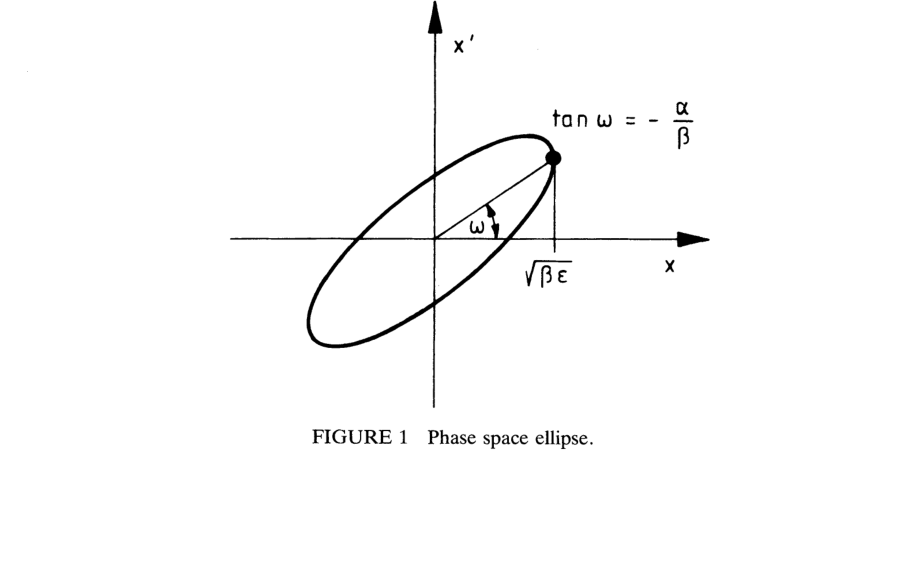
\includegraphics[width=0.72\textwidth]{fig01.png}
\caption{Эллипс в фазовом пространстве. Полуось по $x$ равна
$\sqrt{\beta\varepsilon}$; наклон $\tan\omega=-\alpha/\beta$.}
\label{fig:1}
\end{figure}

Нужны ещё средний набег фазы и разность градиентов:
\begin{equation}
\mu=\tfrac12\bigl[\mu(\delta)+\mu(0)\bigr],
\end{equation}
\begin{equation}
\Delta K=K(\delta)-K(0).
\end{equation}
Из известных соотношений для бетатронных функций\textsuperscript{1} точные
уравнения для $A$ и $B$ (все порядки по $\delta$) таковы:
\begin{equation}
\frac{dB}{ds}=-2A\frac{d\mu}{ds},
\end{equation}
\begin{equation}
\frac{dA}{ds}=+2B\frac{d\mu}{ds}+\sqrt{\beta(0)\beta(\delta)}\,\Delta K.
\end{equation}

Рассмотрим два случая.

\begin{enumerate}
\item[(i)] $\Delta K=0$: участок ахроматический. Из~(6) и~(7) следует
\begin{equation}
\frac{d}{ds}(A^2+B^2)=0,
\end{equation}
\begin{equation}
\frac{d^2 B}{d\mu^2}+4B=0.
\end{equation}
Модуль $\mathbf{W}$ постоянен, сам вектор вращается с удвоенным набегом фазы
$\mu$.

\item[(ii)] $\Delta K\neq 0$: есть локальные изменения градиента. В присутствии
квадруполей и секступолей
\begin{equation}
\Delta K=(-K_0\delta+K_0\delta^2-\cdots+K'_0\eta\delta-K'_0\eta\delta^2+\cdots),
\end{equation}
и локальные ошибки дают толчки $\Delta A$, пропорциональные
$\sqrt{\beta_0\beta_\delta}\,\Delta K\,\Delta s$. Отсюда и из~(10) видно, что
главные источники возмущений $\mathbf{W}$ --- линейных и нелинейных по
$\delta$ --- квадруполи вставок с малой $\beta$, где велики и $K_0$, и $\beta$.
Линейный по $\delta$ вклад секступолей конечен при $\eta\neq 0$ и им управляют
линейной модуляцией $\beta$, порождённой квадруполями. Поскольку секступоли дают
ещё и нелинейности, а управление $\beta$ не всегда удаётся сделать локальной
компенсацией, коррекция хроматичности может оказаться трудной.
\end{enumerate}

\subsection{Уничтожение линейных возмущений}

Линейную по $\delta$ часть $B$ и $A$ [ур.~(2) и~(3)] для возмущений магнитного
канала можно вычислить точно\textsuperscript{4}. Канал между точками 1 и 2
(рис.~\ref{fig:2}): невозмущённое и возмущённое состояния задаются матрицами
$M$ и $M^*$, $\Delta\mu$ --- набег фазы от 1 до 2.

Компоненты в точке 2:
\begin{equation}
B_2=\Gamma_1\cos(2\Delta\mu)+\Sigma_1\sin(2\Delta\mu),
\end{equation}
\begin{equation}
A_2=-\Sigma_1\cos(2\Delta\mu)+\Gamma_1\sin(2\Delta\mu),
\end{equation}
где
\[
\Gamma_1=2\Bigl(c_{11}-\frac{\alpha_1}{\beta_1}c_{12}\Bigr),\qquad
\Sigma_1=\beta_1 c_{21}+2\alpha_1 c_{11}+\frac{1-\alpha_1^2}{\beta_1}c_{12}.
\]
Величины $c_{ij}$ --- элементы $M^{-1}\cdot(M^*-M)$, то есть хроматическое
возмущение $M$ в первом порядке по $\delta$; для квадруполей и секступолей они
считаются явно\textsuperscript{4}. Параметры $\alpha_1$, $\beta_1$ --- значения
$\alpha$ и $\beta$ на входе канала; $\Gamma_1$ и $\Sigma_1$ зависят от силы и
длины элементов, заданных $M$, а также от $\eta$ и $\eta'$.

\begin{figure}[H]
\centering
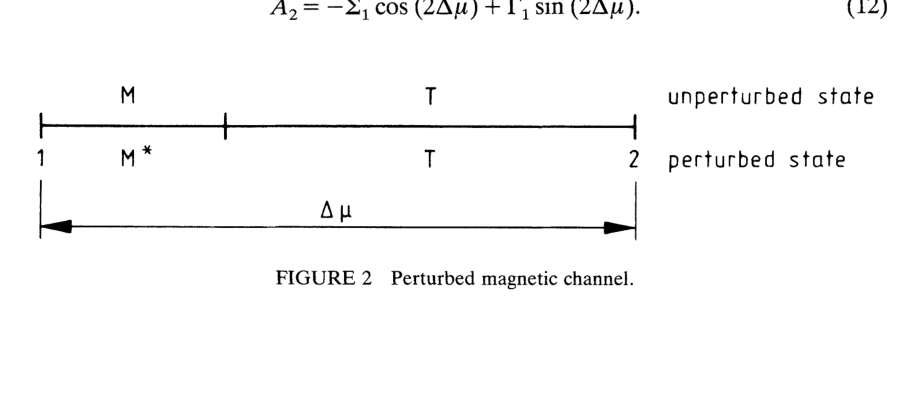
\includegraphics[width=0.85\textwidth]{fig02.png}
\caption{Возмущённый магнитный канал. Сверху --- невозмущённое состояние
($M$, затем $T$), снизу --- возмущённое ($M^*$, тот же $T$).}
\label{fig:2}
\end{figure}

Уравнения~(11) и~(12) снова показывают, что $\mathbf{W}$ вращается с удвоенным
набегом фазы. Ими можно аналитически посчитать эффект семейств
секступолей\textsuperscript{5} в одной точке решётки. Рассмотрим структуру
(например, LEP) из $n$ групп по $k$ ячеек (рис.~\ref{fig:3}); в ней $nk$
секступолей каждого типа (фокусирующих и дефокусирующих). Каждый секступоль даёт
линейный вклад~(11)--(12); полный эффект в точке $P$ --- сумма вкладов (для
$\Delta\mu$ берутся индивидуальные набеги фазы секступолей с рис.~\ref{fig:3}).

\begin{figure}[H]
\centering
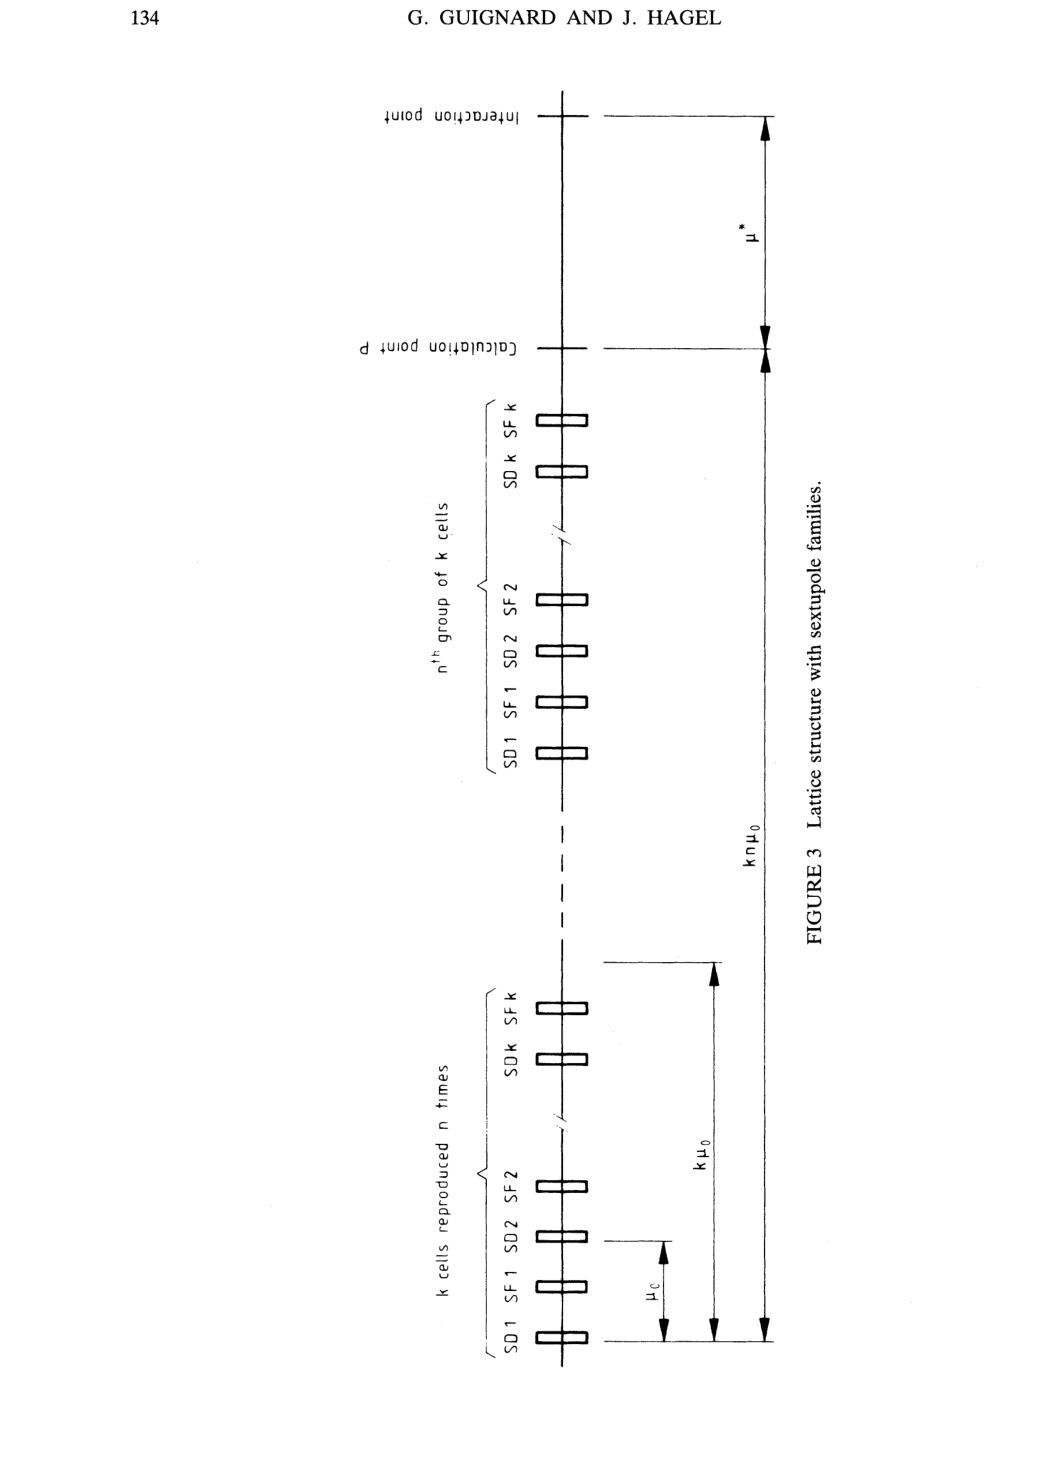
\includegraphics[width=\textwidth]{fig03.png}
\caption{Структура решётки с семействами секступолей. $k$ ячеек, повторённых
$n$ раз (SD1, SF1, \ldots, SD$k$, SF$k$); набеги $\mu_c$ между соседними
секступолями, $k\mu_0$ на группу, $kn\mu_0$ до точки расчёта $P$; далее набег
$\mu^*$ до точки взаимодействия.}
\label{fig:3}
\end{figure}

Суммы синусов и косинусов сводятся к
\begin{equation}
\sum_{j=1}^{n}
\begin{Bmatrix}\cos\\ \sin\end{Bmatrix}(2jk\mu_0)
=
\begin{Bmatrix}\cos\\ \sin\end{Bmatrix}\bigl[(n+1)k\mu_0\bigr]
\frac{\sin(nk\mu_0)}{\sin(k\mu_0)}.
\end{equation}
Отношение синусов в~(13) задаёт условие, при котором эффекты секступолей $n$
групп складываются линейно (когерентно):
\begin{equation}
\frac{\sin(nk\mu_0)}{\sin(k\mu_0)}=\pm n
\quad\text{если}\quad
k\mu_0=\begin{Bmatrix}(2m+1)\pi\\ 2m\pi\end{Bmatrix}.
\end{equation}
При этом условии секступоли эффективнее, и полный вектор $\mathbf{W}$ можно
записать как
\begin{equation}
\begin{cases}
B_P=n\sum_j a_{1j}X_j,\\
A_P=n\sum_j a_{2j}X_j,
\end{cases}
\qquad 1\le j\le 2(k-1).
\end{equation}
Коэффициенты $a_{1j}$, $a_{2j}$ явно выписаны для $\mu_0=60^\circ$ и
$90^\circ$ в работе\textsuperscript{5}. Переменные $X_j$ --- линейные разности
сил секступолей (см.\textsuperscript{5} и табл.~\ref{tab:I}).

Пусть во вставке с малой $\beta$, отстоящей от $P$ (рис.~\ref{fig:3}) на фазу
$\mu^*$, сильные квадруполи создают возмущение
$\mathbf{W}^*=(0,A^*)\approx(0,-\beta_{\max}\ell K)$. В первом приближении этот
вектор поворачивается на $2\mu^*$ между вставкой и $P$ (канал почти
ахроматический), и в точке $P$
\begin{equation}
\begin{cases}
B_I=-A^*\sin(2\mu^*),\\
A_I=+A^*\cos(2\mu^*).
\end{cases}
\end{equation}

Уничтожение линейных по $\delta$ возмущений $\beta$-функции требует, чтобы
векторы~(15) и~(16) были равны и противоположны. Кроме того, из~(1): глобальная
хроматичность обращается в нуль, когда вклад секступолей в интеграл компенсирует
квадруполи. Поэтому коррекция хроматичности первого порядка сводится к трём
уравнениям на каждую поперечную плоскость:
\begin{equation}
(\beta_{x,z}D_x\ell)_{\mathrm{SD}}Y_1+(\beta_{x,z}D_x\ell)_{\mathrm{SF}}Y_2
=-4\pi Q'_{x,z}(\text{квадруполи}),
\end{equation}
\begin{equation}
+A^*_{x,z}\sin(2\mu^*_{x,z})=n\sum_j a_{x,z\,1j}X_j,
\end{equation}
\begin{equation}
-A^*_{x,z}\cos(2\mu^*_{x,z})=n\sum_j a_{x,z\,2j}X_j,
\end{equation}
где $1\le j\le 2(k-1)$, $\ell$ --- длина секступоля, $Y_1$ и $Y_2$ --- суммы сил
SD и SF соответственно.

Линейные возмущения уничтожаются решением этих шести уравнений. Число
независимых переменных зависит от набега фазы на ячейку $\mu_0$, числа $k$
ячеек в группе (рис.~\ref{fig:3}) и кратности $\pi$ в~(14); эти три параметра
связаны. Результаты --- в табл.~\ref{tab:I}. Для набегов LEP $60^\circ$ и
$90^\circ$\textsuperscript{6} первый вариант даёт точную компенсацию линейного
хроматического возмущения в общем случае, второй --- только при определённых
набегах $\mu_x^*$ и $\mu_z^*$ между квадруполями вставки и первым секступолем.

\begin{table}[H]
\centering
\caption{Независимые переменные для уничтожения линейных возмущений.}
\label{tab:I}
\small
\begin{tabular}{@{}llllp{8.2cm}@{}}
\toprule
$2m+1$ или $2m$ & $k$ & $\mu_0$ & $2(k-1)$ & Число независимых переменных ($2k$) \\
\midrule
1 & 2 & $90^\circ$ & 2 &
\textbf{4 переменные:} $Y_1$, $Y_2$,
$X_1=K'_{F1}-K'_{F2}$, $X_2=K'_{D1}-K'_{D2}$.
В принципе недостаточно, но можно использовать также $\mu^*_{x,z}$\textsuperscript{5}. \\[0.6em]
1 & 3 & $60^\circ$ & 4 &
\textbf{6 переменных:} $Y_1$, $Y_2$;
$X_1=K'_{F1}-\tfrac12 K'_{F2}-\tfrac12 K'_{F3}$,
$X_3$ --- то же с $F\to D$;
$X_2=K'_{F2}-K'_{F3}$, $X_4$ --- то же с $F\to D$.
\textbf{Оптимум для линейной задачи.} \\[0.6em]
1 & 4 & $45^\circ$ & 6 &
\textbf{8 переменных:} больше, чем нужно, но фокусировка слабая. \\[0.6em]
3 & 5 & $108^\circ$ & 8 &
\textbf{10 переменных:} большое расстояние между одинаковыми толчками (см.\ далее). \\[0.6em]
2 & 5 & $72^\circ$ & 8 &
\textbf{10 переменных} \\
2 & 7 & $51{,}5^\circ$ & 12 &
\textbf{14 переменных} \\
4 & 9 & $80^\circ$ & 16 &
\textbf{18 переменных} \\
\bottomrule
\end{tabular}

\vspace{0.4em}
{\footnotesize Последние три строки авторы не удерживают: там $k\mu_0$ --- чётное
кратное $\pi$ (см.\ §3.2: для сокращения аберраций выгоднее $k\mu_0=\pi$).}
\end{table}

\section{Нелинейные возмущения и численные инструменты}

Как видно из раздела~2, главные источники хроматических ошибок --- вставки с
малой $\beta$. Обычно они расположены в середине протяжённой области без
дисперсии $D_x$, поэтому компенсацию делают секступолями, установленными в
решётке ($D_x\neq 0$), как на рис.~\ref{fig:3}. В дрейфе между вставкой и
решёткой вектор $\mathbf{W}^*$ в первом приближении вращается (§2.2), но
развиваются нелинейности по $\delta$. В решётке вклад каждого секступоля
складывается с остальными и вращается с набегом фазы, но появляются и
нелинейности по $\delta$. Наконец, наличие секступолей означает нелинейные силы
по поперечным координатам $x$ и $z$.

\subsection{Нелинейности и характерные величины}

Упомянутые нелинейности по $\delta$ бывают двух видов: (i)~амплитудные, обычно
слабые, и (ii)~фазовые, которые велики и следуют за разбросом фазы. Нелинейности,
возникающие в решётке и в дрейфе у вставки, разумеется, различны. Чтобы это
показать, изобразим векторы $\mathbf{W}$, протреканные из решётки и из вставки
до точки $P$ (рис.~\ref{fig:3}), как функции $\delta$. Рис.~\ref{fig:4} ---
результаты для структуры LEP. Силы секступолей посчитаны, как в §2.2, так что
два вектора $\mathbf{W}$ равны и противоположны при $\delta=0$; ожидалось, что
это приближённо сохранится при малых $\delta\neq 0$. Рис.~\ref{fig:4} показывает,
однако, что при $|\delta|$ от $0{,}5\%$ до $1{,}5\%$ компенсация плохая. Также
видно, что доминируют фазовые нелинейности.

\begin{figure}[H]
\centering
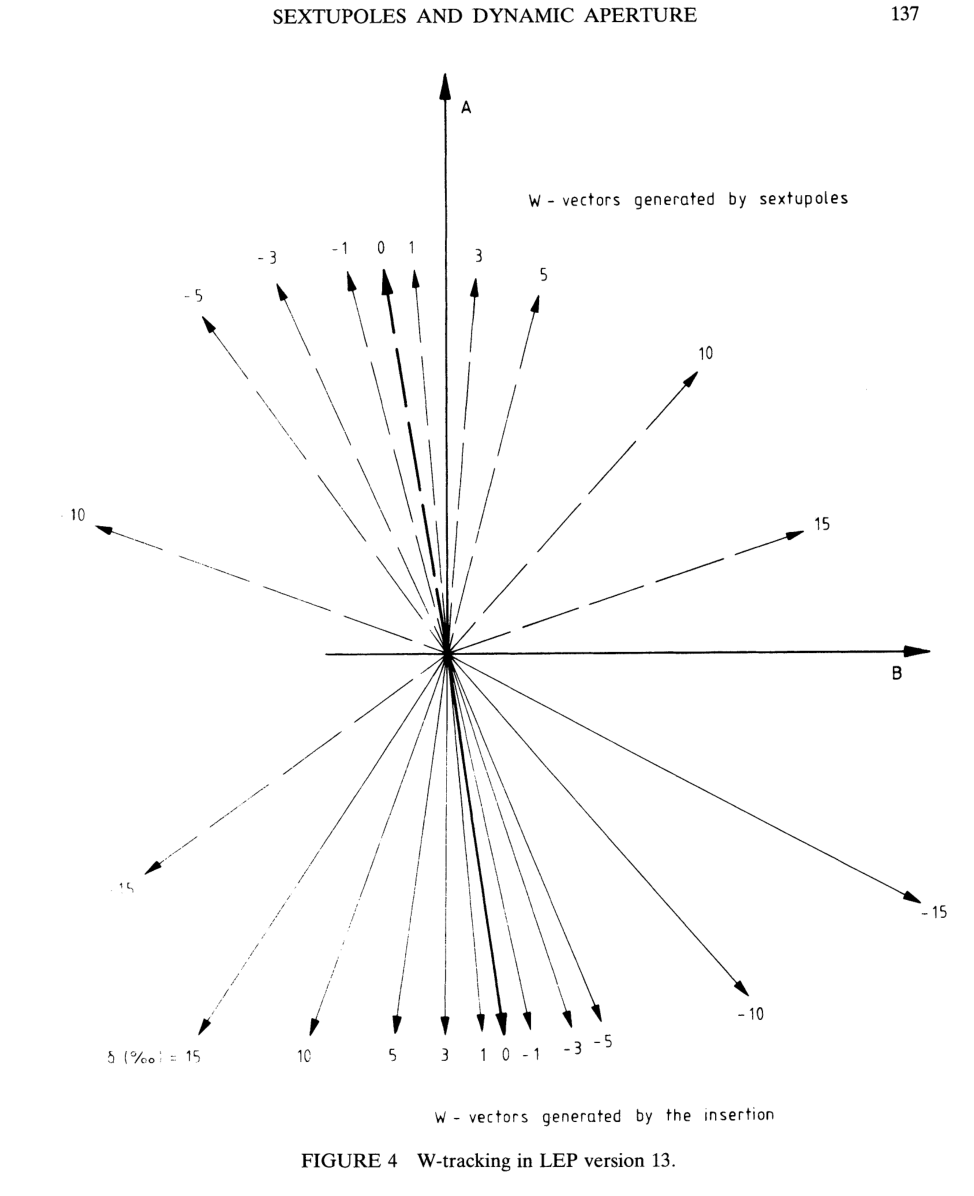
\includegraphics[width=0.88\textwidth]{fig04.png}
\caption{Трекинг векторов $\mathbf{W}$ в LEP, версия~13. Сверху --- векторы,
порождённые секступолями; снизу --- векторы, порождённые вставкой. Подписи у
стрелок --- $\delta$ в промилле.}
\label{fig:4}
\end{figure}

Нелинейные поперечные силы по $x$ и $z$ дают нелинейные толчки бетатронного
движения: резонансы, связь $x$--$z$, неустойчивости и раздувание пучка.

Важно определить величины, характеризующие эти нелинейные эффекты. Для
нелинейностей по $\delta$ это, например, зависимости частоты и бетатронной
функции от $\delta$. На рис.~\ref{fig:5} --- вариации, полученные для
LEP\textsuperscript{7}. Рисунок показывает, что линейная коррекция достигнута и
что неустойчивость на целой частоте наступает при $\delta=1{,}8\%$, но не даёт
явных указаний на \emph{качество} коррекции. Для нелинейных сил по $x$ и $z$
вычислимы коэффициенты возбуждения и стабилизации резонансов третьего
порядка\textsuperscript{8} и четвёртого порядка\textsuperscript{9} (последние ---
из-за распространения секступольных эффектов через нелинейные колебания
траектории).

\begin{figure}[H]
\centering
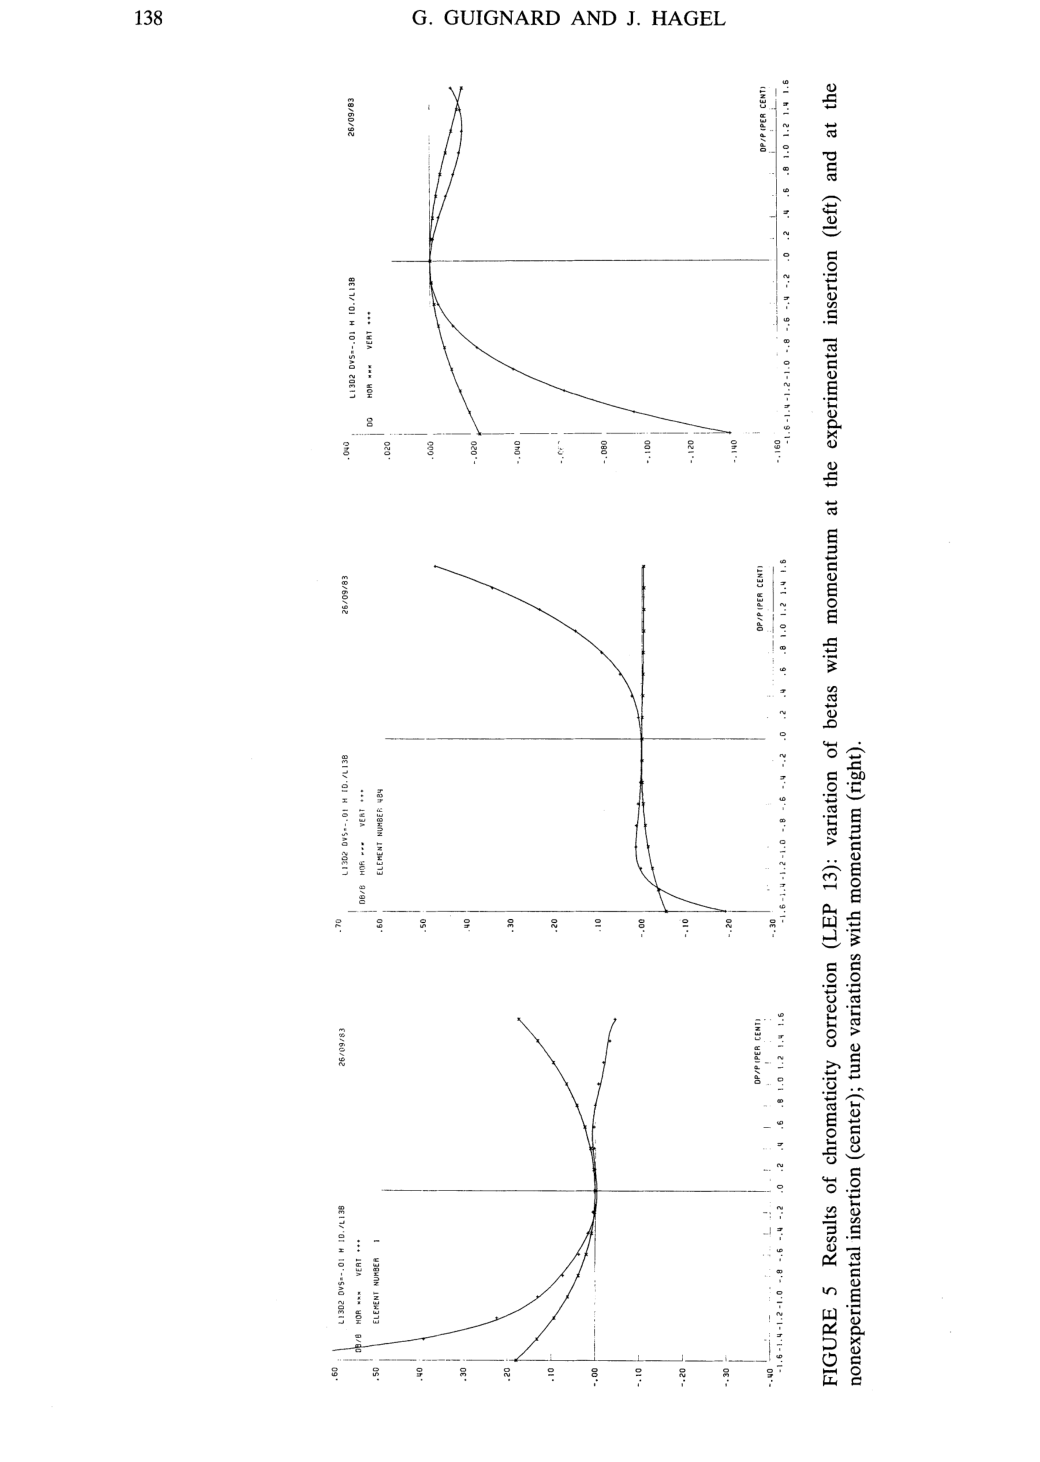
\includegraphics[width=\textwidth]{fig05.png}
\caption{Результаты коррекции хроматичности (LEP~13): вариация $\beta$ с
импульсом на экспериментальной вставке (слева) и на неэкспериментальной
(центр); вариации частоты с импульсом (справа).}
\label{fig:5}
\end{figure}

Один из способов глобально описать все эффекты и оценить качество коррекции ---
смотреть на динамическую апертуру. Динамическая апертура $d_y$ ($y$ есть $x$
или $z$) и динамический аксептанс $A_y=d_y^2/\beta_y$ описывают бетатронные
амплитуды, при которых частицы могут циркулировать в машине неограниченно долго,
как функции отклонения импульса $\delta$. Динамическая апертура соответствует
начальным амплитудам, ниже которых бетатронное движение устойчиво, то есть
остаётся ограниченным. Для излучающих электронов условие ограниченности должно
выполняться лишь в течение времени, сравнимого со временами затухания.

В принципе устойчивая область --- это объём в пространстве $(E_x,E_z,\delta)$,
центрированный около начала координат. $E_x$ и $E_z$ --- эмиттансы, связанные с
амплитудами бетатронных колебаний, $\delta$ --- относительная амплитуда
синхротронных колебаний. Ищут наибольшую поверхность простой формы, лежащую
внутри устойчивой области, тем самым отбрасывая острова устойчивости вдали от
начала. Иногда для упрощения показывают только сечения устойчивого объёма
(например, сечение $E_z=\tfrac12 E_x$, отвечающее полной связи в электронных
машинах).

До сих пор динамическую апертуру можно было получить только трекингом траекторий
достаточно долго: одно время затухания для электронов и время, большое по
сравнению с синхротронным периодом, для протонов. Однако одновременно искали
аналитические инструменты --- и чтобы прояснить задачу динамической апертуры, и
чтобы сократить время трекинга, необходимое для адронов.

\subsection{Зависимость от расстановки секступолей}

Два нелинейных толчка одинаковой силы от секступолей $S_1$ и $S_2$ могут
уничтожить друг друга, если разность фаз равна нечётному кратному $\pi$ и между
ними нет других нелинейных возмущений (рис.~\ref{fig:6}).

\begin{figure}[H]
\centering
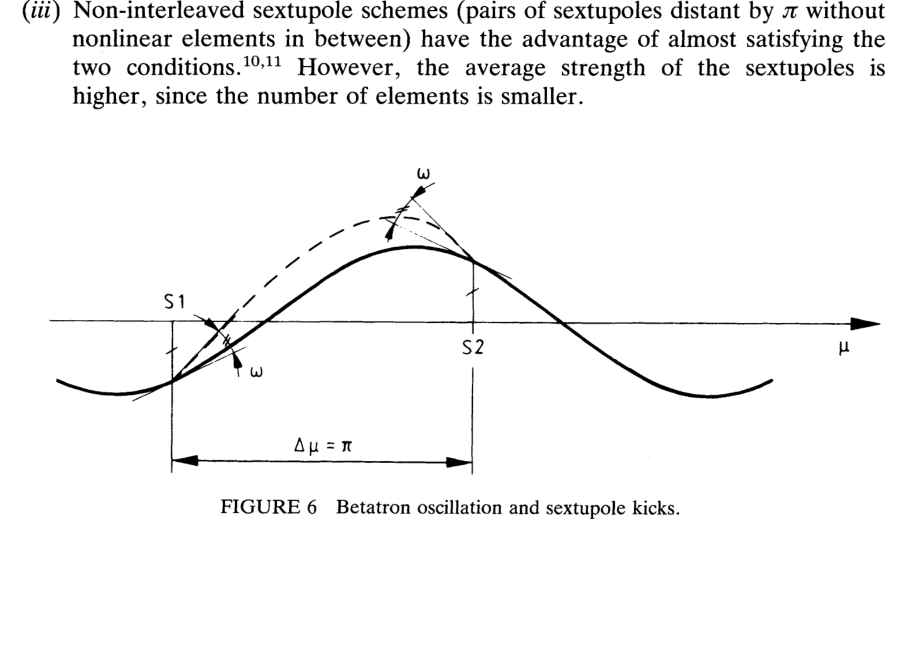
\includegraphics[width=0.78\textwidth]{fig06.png}
\caption{Бетатронное колебание и толчки секступолей. При $\Delta\mu=\pi$ второй
толчок компенсирует первый.}
\label{fig:6}
\end{figure}

При этих условиях поперечные аберрации уничтожаются во всех порядках. Однако
$\Delta\mu=(2m+1)\pi$ выполняется лишь при одном значении $\delta$ (именно
$\delta=0$), и на практике трудно избежать других секступолей на таком
расстоянии. Следствия таковы:

\begin{enumerate}
\item[(i)] В принципе выгодно делать линейную коррекцию при $k\mu_0=\pi$, то есть
$(2m+1)=1$ [в ур.~(14)].
\item[(ii)] Чередующиеся (interleaved) схемы, как на рис.~\ref{fig:3}, не
удовлетворяют второму условию выше; зато средняя сила секступолей ниже.
\item[(iii)] Нечередующиеся (non-interleaved) схемы --- пары секступолей на
расстоянии $\pi$ без нелинейных элементов между ними --- почти удовлетворяют
обоим условиям\textsuperscript{10,11}. Однако средняя сила секступолей выше,
поскольку элементов меньше.
\end{enumerate}

Качественные черты динамической апертуры для этих двух схем можно набросать
(рис.~\ref{fig:7} --- примеры для конфигураций LEP с разными рабочими точками).

\textit{Схема~(iii).} Поскольку $\Delta\mu=\pi$ при $\delta=0$, величина $d_y$
очень велика в начале (но конечна из-за конечной длины секступоля). Так как силы
велики и $\Delta\mu\neq\pi$ при $\delta\neq 0$, $d_y$ быстро падает с $\delta$.

\begin{figure}[H]
\centering
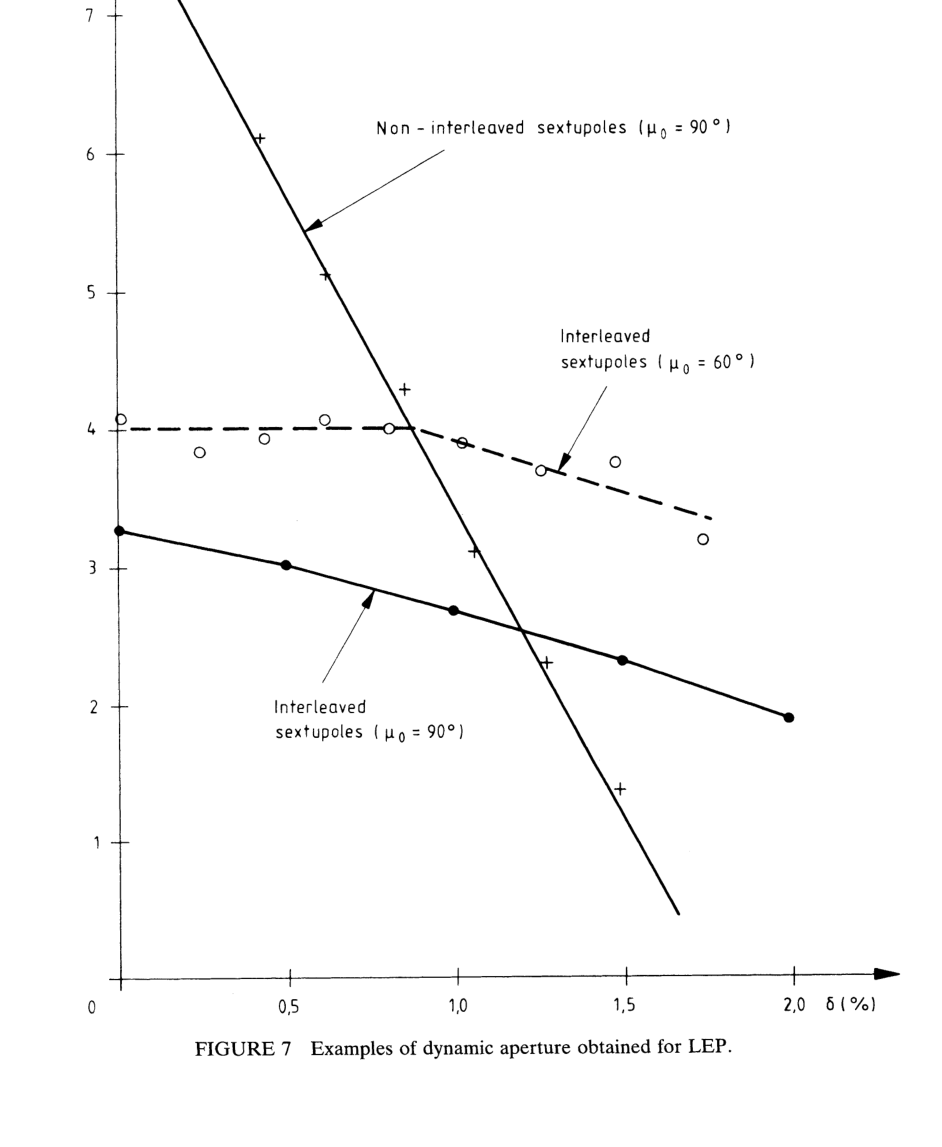
\includegraphics[width=0.82\textwidth]{fig07.png}
\caption{Примеры динамической апертуры, полученные для LEP. По вертикали
$10^3\sqrt{A}$ (м$^{1/2}$), по горизонтали $\delta$~(\%). Сплошная с плюсами ---
нечередующиеся секступоли ($\mu_0=90^\circ$); штриховая с кружками ---
чередующиеся ($\mu_0=60^\circ$); сплошная с точками --- чередующиеся
($\mu_0=90^\circ$).}
\label{fig:7}
\end{figure}

\textit{Схема~(ii).} Из-за секступолей внутри пары элементов, разделённых на
$\pi$, $d_y$ в начале меньше. Поскольку силы ниже, можно ограничить падение
$d_y$ с $\delta$.

Заметим, что чередующиеся секступоли с <<высокими>> силами --- крайний случай,
сочетающий недостатки. Это аргумент против локальной компенсации возмущений
вставки чередующимися секступолями, например на краях решётки.

Интересно упомянуть дополнительные средства\textsuperscript{12,13} для изменения
производных частоты высокого порядка по $\delta$. Во-первых, набег фазы $\mu^*$
(§2.2) можно использовать при $\mu_0\neq 90^\circ$, чтобы менять модуляцию
$\beta$ на секступолях при $\delta\neq 0$. Во-вторых, одно семейство секступолей
(члены которого все эквивалентны для линейной коррекции) можно разбить на
подгруппы с заведомо разной модуляцией $\beta$ при $\delta\neq 0$.

\subsection{Коррекция хроматичности и компьютерные расчёты}

Опишем на примере, как считалась коррекция хроматичности LEP и какие программы
использовались.

Задавшись набегом фазы на ячейку решётки $\mu_0$, считают линейную коррекцию,
удовлетворяя условию $k\mu_0=(2m+1)\pi$ [ур.~(14)] и при необходимости используя
переменную $\mu^*$ (рис.~\ref{fig:3}). Затем программа HARMON\textsuperscript{14}
ищет силы секступолей, минимизирующие линейные возмущения, а также нелинейности
по $\delta$ ($Q''$, $Q'''$, $\beta''$, \ldots) и возбуждения резонансов из §3.1.
Чтобы показать, что линейная коррекция --- хорошая стартовая точка,
табл.~\ref{tab:II} сравнивает силы HARMON с решением линейной задачи для LEP с
$\mu_0=90^\circ$ и чередующимися секступолями\textsuperscript{15}.

Оптическая программа MAD\textsuperscript{16} позволяет затем для полученного
решения посчитать вариации бетатронных параметров (частот и $\beta$) с $\delta$
(см.\ рис.~\ref{fig:5}), чтобы проверить линейную коррекцию и увидеть остаточные
эффекты нелинейностей по $\delta$.

Следуя идее §3.1, программа PATRICIA\textsuperscript{17} трекает траектории при
разных начальных горизонтальных амплитудах $x$ ($x'$ всегда нуль) и разных
амплитудах $\delta$ синхротронных колебаний. Трекинг начинается на вставке с
малой $\beta$ и идёт несколько сотен оборотов в предположении
$E_z=\tfrac12 E_x$. Для каждого $\delta$ программа указывает, остаётся ли
движение ограниченным за рассматриваемое время, и выдаёт аксептанс $A_x$ или
величину $(A_x)^{1/2}$ (§3.1). Кривая $(A_x)^{1/2}$ как функция $\delta$ и есть
динамическая апертура, определённая в §3.1 (рис.~\ref{fig:7}). Как правило,
кривая не показывает узких провалов в местах резонансов: синхротронное движение
ослабляет эффекты. Однако осмотр траекторий в фазовом пространстве может выявить
острова устойчивости, связанные с резонансами и зависимостью частоты от
амплитуды (рис.~\ref{fig:8}). Когда горизонтальная амплитуда близка к границе
устойчивости, сепаратриса этих резонансов может стать отчётливо видна
(рис.~\ref{fig:9}).

\begin{table}[H]
\centering
\caption{Силы секступолей, в м$^{-3}$, для LEP с $90^\circ$ на ячейку.}
\label{tab:II}
\begin{tabular}{@{}lcccc@{}}
\toprule
 & $K'_{SF1}$ & $K'_{SF2}$ & $K'_{SD1}$ & $K'_{SD2}$ \\
\midrule
Линейная компенсация & $0{,}216$ & $0{,}141$ & $0{,}288$ & $0{,}128$ \\
HARMON & $0{,}209$ & $0{,}125$ & $0{,}260$ & $0{,}143$ \\
\bottomrule
\end{tabular}
\end{table}

\begin{figure}[H]
\centering
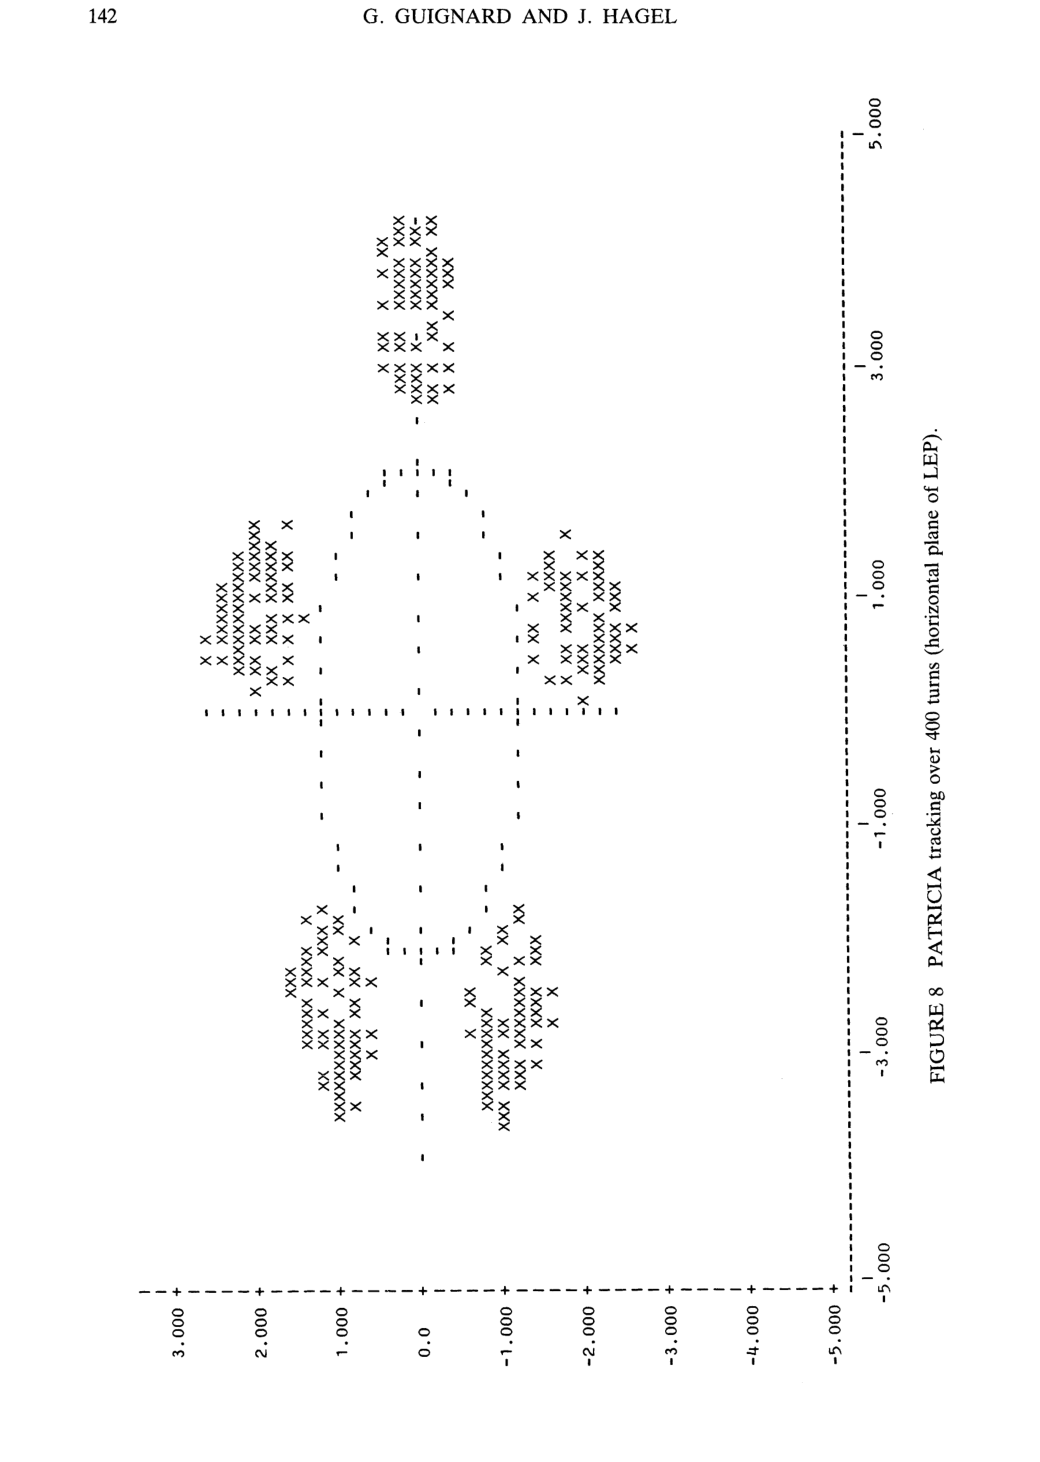
\includegraphics[width=0.92\textwidth]{fig08.png}
\caption{Траектории в фазовом пространстве: острова устойчивости, связанные с
резонансами и зависимостью частоты от амплитуды.}
\label{fig:8}
\end{figure}

\begin{figure}[H]
\centering
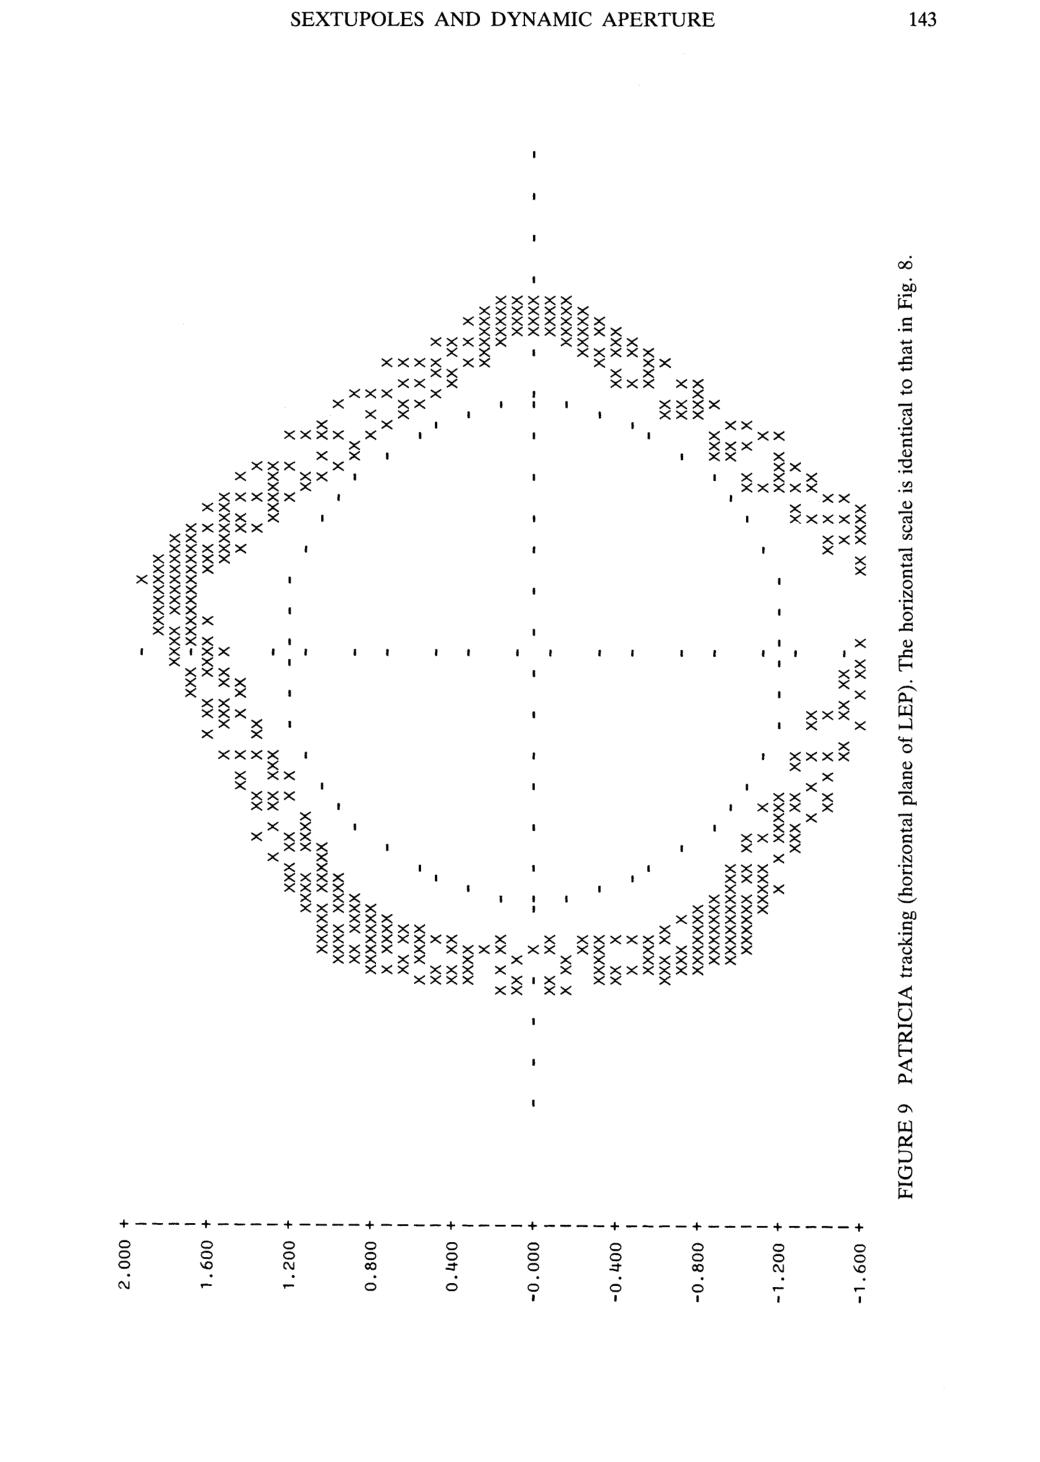
\includegraphics[width=0.92\textwidth]{fig09.png}
\caption{Фазовое пространство вблизи границы устойчивости: видна сепаратриса
резонансов.}
\label{fig:9}
\end{figure}

\section{Аналитический подход в гамильтоновом формализме}

Как сказано в §3.1, аналитические инструменты также очень полезны для работы с
нелинейными силами секступолей, введённых для коррекции хроматичности. В этой
работе рассматриваются два формализма. Первый, основанный на классическом
гамильтоновом подходе, описан здесь; второй, исходящий непосредственно из
дифференциального уравнения, --- предмет раздела~5. Обсуждаются возможные
приложения и ограничения обоих формализмов, имея в виду вопрос динамической
апертуры.

\subsection{Нелинейные возмущения в двух измерениях}

Основные принципы гамильтонова подхода описаны, например, в
работе\textsuperscript{18} для одномерного бетатронного движения. Здесь нас
интересует двумерное бетатронное движение, и применяется общее изложение
работ\textsuperscript{9,19,20}.

Начнём с линейного <<невозмущённого>> движения, которое описывается следующими
уравнениями и гамильтонианом $H$ (независимая переменная --- продольная
координата $s$):
\begin{equation}
\begin{aligned}
x''+K_1 x&=0,\\
z''+K_2 z&=0,\\
H_0&=\tfrac12(K_1 x^2+K_2 z^2+p_x^2+p_z^2).
\end{aligned}
\end{equation}
Показано\textsuperscript{1}, что общее решение имеет вид
\begin{equation}
\begin{aligned}
x&=A_x\sqrt{\beta_x}\exp(i\mu_x),\\
z&=A_z\sqrt{\beta_z}\exp(i\mu_z).
\end{aligned}
\end{equation}
В присутствии нелинейных полей возмущённое движение можно записать так\textsuperscript{20}:
\begin{equation}
\begin{aligned}
x''+K_1 x&=-\frac{\partial H_1}{\partial x},\\
z''+K_2 z&=-\frac{\partial H_1}{\partial z},\\
H_1=\sum_N H^{(N)}
&=\sum_{k_1+k_2=N}\frac{\pm 1}{k_1!\,k_2!}\,K_{z,x}^{(N-1)}x^{k_1}z^{k_2}.
\end{aligned}
\end{equation}
Здесь $H_1$ --- гамильтониан возмущения, а $K_{z,x}^{(N-1)}$ --- нормированные
производные порядка $N-1$ компонент поля $B_z$ или $B_x$. Если теперь для полного
движения ($H=H_0+H_1$) ввести переменные действие--угол $I_x$, $I_z$, $\Phi_x$,
$\Phi_z$ и независимую переменную $\theta$ (геометрический угол относительно
центра машины), две части $H$ записываются так\textsuperscript{20}:
\begin{equation}
H_0=Q_x I_x+Q_z I_z
\end{equation}
и
\begin{equation}
H_1=\sum_{jklm}h_{jklm}\,I_x^{(j+k)/2}I_z^{(l+m)/2}
\exp\bigl\{i\bigl[(j-k)(\Phi_x+Q_x\theta)+(l-m)(\Phi_z+Q_z\theta)\bigr]\bigr\},
\end{equation}
где
\begin{align*}
h_{jklm}=h_C
&=\frac{1}{2^{(N+1)/2}j!\,k!\,l!\,m!}\,\frac{1}{2\pi}
\int_0^{2\pi}
\Bigl(\frac{\beta_x}{R}\Bigr)^{(j+k)/2}
\Bigl(\frac{\beta_z}{R}\Bigr)^{(l+m)/2}
K_{z,x}^{(N-1)}\,d\theta\\
&\quad\times\exp\bigl\{i\bigl[(j-k)(\mu_x-Q_x\theta)+(l-m)(\mu_z-Q_z\theta)\bigr]\bigr\}.
\end{align*}
Здесь $Q_x$, $Q_z$ --- частоты (тюны), $C$ --- набор индексов $jklm$. В частном
случае $H_1\equiv 0$ величина $H_0$ --- константа движения, задающая
инвариантные кривые. В интересующем нас случае $H_1\neq 0$ метод состоит в
поиске канонического преобразования, порождающего новый гамильтониан $G$, либо
почти не зависящий от $\theta$ для низких частот, либо точно не зависящий от
$\theta$ в первом порядке по возмущению\textsuperscript{20,21}. Это
преобразование задаётся производящей функцией
\begin{equation}
S_{\mathrm{tot}}(\Phi_x,J_x,\Phi_z,J_z,\theta)
=\Phi_x J_x+\Phi_z J_z+S(\Phi_x,J_x,\Phi_z,J_z,\theta).
\end{equation}
По определению связь старых переменных $(\Phi_x,I_x,\Phi_z,I_z)$ с новыми
$(\Psi_x,J_x,\Psi_z,J_z)$ и старого гамильтониана с новым такова:
\begin{equation}
\begin{aligned}
\Psi_x&=\Phi_x+\partial_{\Phi}S\big|_{J_x},&
\Psi_z&=\Phi_z+\partial_{\Phi}S\big|_{J_z},\\
I_x&=J_x+\partial_{\Phi}S\big|_{\Phi_x},&
I_z&=J_z+\partial_{\Phi}S\big|_{\Phi_z},\\
G&=H+\partial_\theta S.
\end{aligned}
\end{equation}
Здесь $\partial_\Phi S$, $\partial_J S$ и $\partial_\theta S$ --- частные
производные по $\Phi$, $J$ и $\theta$. Формально $S$ записывается как $H_1$
[ур.~(24)], где $h_C$ заменено на $s_C$, а $I_{x,z}$ --- на $J_{x,z}$. Аналогично
новый гамильтониан $G$ имеет ту же форму, что $H$, с заменами $h_C\to g_C$,
$I_{x,z}\to J_{x,z}$, $\Phi_{x,z}\to\Psi_{x,z}$. Три функции $S$, $H$ и $G$ имеют
одинаковый вид, но разные переменные. Выражая все их через переменные $S$, нужно
разложить остальные переменные в ряд Тейлора по определениям~(26). Делая это и
пользуясь последним из~(26), получаем для нового гамильтониана $G$
\begin{align}
G(\Psi_x,J_x,\Psi_z,J_z)
&=G(\Phi_x,J_x,\Phi_z,J_z)
+\partial_{\Psi_x}G\,\partial_{J_x}S
+\partial_{\Psi_z}G\,\partial_{J_z}S+\cdots \nonumber\\
&=\underline{H_0(J_x,J_z)}
+\underline{Q_x\partial_{\Phi_x}S}
+\underline{Q_z\partial_{\Phi_z}S}+\cdots
+\underline{\partial_\theta S}\nonumber\\
&\quad+\underline{H_1(\Phi_x,J_x,\Phi_z,J_z)}
+\partial_{I_x}H_1\,\partial_{\Phi_x}S
+\partial_{I_z}H_1\,\partial_{\Phi_z}S+\cdots,
\end{align}
напоминая, что $Q=\partial H_0/\partial I$. Поскольку возмущение входит в $G$,
$S$ и $H_1$, произведения двух частных производных --- второго порядка по
возмущению, и единственные члены первого порядка --- подчёркнутые в~(27). Для
циклических ускорителей все функции периодичны по $\theta$, $\Phi_x$ и $\Phi_z$
с периодом $2\pi$. Поэтому их можно разложить в ряд Фурье, например
\begin{equation}
H_1=\sum_{C,p=-\infty}^{\infty}
h_{Cp}\,I_x^{(j+k)/2}I_z^{(l+m)/2}
\exp\bigl\{i\bigl[(j-k)(\Phi_x+Q_x\theta)+(l-m)(\Phi_z+Q_z\theta)-p\theta\bigr]\bigr\}.
\end{equation}
Аналогичные выражения пишутся для $S$ и для $G-H_0$ с коэффициентами $s_{Cp}$ и
$g_{Cp}$. Подставляя их в~(27) и оставляя только члены первого порядка,
получаем
\begin{equation}
g_{Cp}=i(j-k)Q_x s_{Cp}+i(l-m)Q_z s_{Cp}-i p s_{Cp}+h_{Cp},
\end{equation}
где $C$ снова заменяет четыре индекса $j,k,l,m$. Производящую функцию $S$
[ур.~(26)] можно выбрать произвольно, лишь бы выполнялось~(29). Решим~(29)
относительно $s_{Cp}$:
\begin{equation}
s_{Cp}=i\frac{h_{Cp}-g_{Cp}}{(j-k)Q_x+(l-m)Q_z-p}.
\end{equation}
Это ключевое уравнение. Каноническое преобразование $I\to J$, $\Phi\to\Psi$
должно оставаться конечным, а сходимость $S$ требует ограниченности $s_{Cp}$.
Различаются два случая.

\begin{enumerate}
\item[(i)] \textbf{Резонансный подход.} Знаменатель~(30) обращается в нуль;
удерживаются низкочастотные члены типа $n_x Q_x+n_z Q_z=p$, отвечающие
нелинейным резонансам. Поскольку $s_{Cp}$ должно быть ограниченным, числитель
должен быть нулём, то есть $h_{Cp}=g_{Cp}$. Тогда $s_{Cp}$ --- константа,
выбираемая равной нулю. Члены первого порядка $g_{Cp}$ нового гамильтониана
ненулевые, и применяется известная теория возмущений первого
порядка\textsuperscript{8,9,19,20}: линии одиночных резонансов, коэффициенты
возбуждения и стабилизации, ширины, резонансные кривые, сепаратрисы.

\item[(ii)] \textbf{Глобальный подход.} Частоты $Q_x$, $Q_z$ таковы, что рабочая
точка далека от всякого сильного резонанса и может быть близка лишь к слабым,
пренебрежимым. Тогда знаменатель~(30) всегда отличен от нуля, и можно положить
$g_{Cp}=0$. Все члены первого порядка нового гамильтониана исчезают, а
зависимость от $\theta$ переносится во второй порядок по
возмущению\textsuperscript{21}. Этот подход позволяет изучать движение между
сильными резонансами и оценивать искажения инвариантных кривых и модуляцию
амплитуд --- в известных пределах применимости.
\end{enumerate}

\subsection{Резонансный подход}

Как объяснено выше, коэффициенты $g_{Cp}$ берутся равными $h_{Cp}$. В полном
выражении нового гамильтониана [ур.~(27)] нужно вернуть члены высших порядков,
отброшенные при выводе~(30). Тогда $G$ имеет вид
\begin{align}
G&=H_0+\sum_{C,p}h_{Cp}\,J_x^{(j+k)/2}J_z^{(l+m)/2}\exp i(\cdots)\nonumber\\
&\quad+\sum_{C'q'C''q''}h_{C'q'}h_{C''q''}\,f_1(C',q',C'',q'')
J_x^{(j'+k'+j''+k''-2)/2}J_z^{(l'+m'+l''+m'')/2}\exp i(\cdots)\nonumber\\
&\quad+\sum_{C''q''C'q'}h_{C'q'}h_{C''q''}\,f_2(C'',q'',C',q')
J_x^{(j'+k'+j''+k'')/2}J_z^{(l'+m'+l''+m''-2)/2}\exp i(\cdots)\nonumber\\
&\quad+O(h^3).
\end{align}
Функции $f_1$ и $f_2$ индексов и фаз явно не выписываются. Для возмущений первого
порядка степени $N$ по определению
$j+k+l+m=j'+k'+l'+m'=j''+k''+l''+m''=N$. Тогда члены двойных сумм имеют степень
по амплитуде
\begin{equation}
j'+k'+j''+k''+l'+m'+l''+m''-2=2(N-1).
\end{equation}
Следовательно, секступоли, возбуждающие резонансы третьего порядка ($N=3$) за
счёт возмущений первого порядка, возбуждают также резонансы четвёртого порядка
($2N-2=4$) за счёт возмущений второго порядка. Физически: колебания траектории
из-за нелинейных толчков распространяются по кольцу и влияют на толчки других
секступолей. Разумеется, секступоли возбуждают и резонансы ещё более высоких
порядков, связанные с отброшенными в~(31) членами.

Этот подход используется в программе HARMON\textsuperscript{14}, которая
подбирает силы секступолей, минимизируя неблагоприятные эффекты данной
квадрупольно-секступольной конфигурации. Основной принцип --- минимизировать
заданный набор коэффициентов $h_{Cp}$. Например, коэффициенты возбуждения
третьего порядка (по амплитуде) $h_{1020}$, $h_{1002}$ и $h_{1011}$ минимизируют
из-за связанных движений, тогда как $h_{3000}$ и $h_{2100}$ менее важны.
Коэффициенты возбуждения четвёртого порядка косвенно уменьшаются (произведения
$h$) и вычисляются.

Уравнения движения
\begin{equation}
\begin{aligned}
\frac{d\Psi_x}{d\theta}&=\frac{\partial G}{\partial J_x},&
\frac{dJ_x}{d\theta}&=-\frac{\partial G}{\partial\Psi_x},\\
\frac{d\Psi_z}{d\theta}&=\frac{\partial G}{\partial J_z},&
\frac{dJ_z}{d\theta}&=-\frac{\partial G}{\partial\Psi_z}
\end{aligned}
\end{equation}
позволяют затем выразить вариации частот и амплитуд с $\delta$, а также
зависимость частоты от амплитуды. Например, в горизонтальной плоскости
\begin{equation}
Q_x=Q_{x0}+\frac{d\Psi_x}{d\theta}=Q_{x0}+\frac{\partial G}{\partial J_x}.
\end{equation}
Из~(31) частоту можно записать
\begin{equation}
Q_x=Q_{x0}+\sum_{r,s}J_x^{r-1}J_z^{s}
\bigl[r h_{rrss0}+f(C',C'',q',q'')h_{C'q'}h_{C''q''}\bigr],
\end{equation}
где $f$ --- функция индексов с $(j'+k'+j''+k''-4)/2=r-1$ и
$(l'+m'+l''+m''-4)/2=s$. Два частных примера:

\begin{enumerate}
\item[(i)] Член~(35) при $r=1$, $s=0$:
\begin{equation}
h_{11000}-4\sum_q\Biggl(
\frac{h_{2000q}h_{0200,-q}}{2Q_x-q}
+\frac{h_{1000q}h_{1200,-q}}{Q_x-q}\Biggr).
\end{equation}
Сумма даёт зависимость от $\delta$ в силу определения $h$ [ур.~(24)].
Коэффициент $h_{1000q}$ содержит дипольное поле $B$, которому отвечают
$B'\eta\delta$ и $\tfrac12 B''\eta^2\delta^2$ в квадруполях и секступолях
соответственно. Производная $B'$ входит в $h_{2000q}$, а секступоли дают вклад
$B''\eta\delta$. Тем самым зависимость частоты от $\delta$ и $\delta^2$
вычислима.

\item[(ii)] Член~(35) при $r=2$, $s=0$:
\begin{equation}
h_{22000}-9\sum_q\Biggl(
\frac{h_{3000q}h_{0300,-q}}{3Q_x-q}
+\frac13\frac{h_{2100q}h_{1200,-q}}{Q_x-q}\Biggr).
\end{equation}
Все $h$ в сумме содержат $B''$, зависимости от $\delta$ нет. Но при $r=2$
вариация частоты пропорциональна $J_x$ в~(35), и зависимость от амплитуды
вычислима.
\end{enumerate}

Минимизируя некоторые $h_{Cq}$, можно в известной мере управлять вариациями
частоты --- это и делает HARMON\textsuperscript{14}. Кроме того, резонансный
подход позволяет подробно изучать изолированные резонансы, возбуждаемые
секступолями. Вблизи одного из них можно анализировать неподвижные точки,
резонансные кривые и сепаратрисы\textsuperscript{8,9,19,20}, получая сведения о
неограниченности движения. Начальные условия $(x_0,x'_0,z_0,z'_0)$, при которых
достигаются сепаратрисы, дают динамическую апертуру из §3.1. Однако это верно
лишь в узком диапазоне частот вблизи резонансной линии, как позже показано
(рис.~\ref{fig:13}) для одномерного движения. Динамическая апертура вдали от
сильных резонансов требует других подходов (см.\ ниже).

\subsection{Глобальный подход}

В §4.2 можно было подбирать силы секступолей, минимизируя коэффициенты
возбуждения, и получать сведения о границах устойчивости вблизи сильных
резонансов. Но нельзя было сказать ничего о частотах вдали от резонансных
значений и о том, действуют ли два или более резонанса совместно. В анализе
нелинейного движения нас главным образом интересуют искажения инвариантов и
биения амплитуды при частотах вдали от сильных резонансов. Здесь можно
попробовать глобальный подход\textsuperscript{21}.

Поскольку $g_{Cp}=0$, производящая функция имеет вид
\begin{equation}
S=i\sum_{C,p}\frac{h_{Cp}}{Q-p}\,J_x^{(j+k)/2}J_z^{(l+m)/2}
\exp\bigl\{i\bigl[(j-k)\Phi_x^*+(l-m)\Phi_z^*-p\theta\bigr]\bigr\},
\end{equation}
где $Q=(j-k)Q_x+(l-m)Q_z$ и $\Phi_{x,z}^*=\Phi_{x,z}+Q_{x,z}\theta$. Разлагая
Тейлором переход от $\Phi_{x,z}$ к $\Psi_{x,z}$ и отбрасывая второй порядок по
возмущению, подставляем $S$ в~(26). Для старой горизонтальной переменной
действия получаем, например,
\begin{equation}
I_x=J_x-\sum_{C,p}\frac{(j-k)h_{Cp}}{Q-p}\,J_x^{(j+k)/2}J_z^{(l+m)/2}
\exp\bigl\{i\bigl[(j-k)\Psi_x^*+(l-m)\Psi_z^*-p\theta\bigr]\bigr\},
\end{equation}
где $\Psi_{x,z}^*=\Psi_{x,z}+Q_{x,z}\theta$. Бесконечные суммы по гармонике $p$
в~(39) считаются по формуле
\begin{equation}
\sum_p\frac{e^{ip\theta}}{Q-p}=\frac{\pi}{\sin(\pi Q)}\exp\bigl[-iQ(\pi-\theta)\bigr].
\end{equation}
Новый гамильтониан $G$ содержит только второй порядок по $h$, но всё ещё зависит
от $\theta$. Эту остаточную зависимость снимают усреднением по $\theta$, то есть
удерживая только низкочастотные члены. Тогда $G$ не зависит от фаз $\Psi_x$,
$\Psi_z$:
\begin{equation}
\bar G=Q_x J_x+Q_z J_z+\sum_{m,n}B_{mn}J_x^{m/2}J_z^{n/2}.
\end{equation}
Следовательно, $\bar G$ --- константа движения, как и $J_x$, $J_z$, в силу
уравнений движения~(33). Константа $\bar G$ даёт новый инвариант: первые два
члена~(41) отвечают эллипсу линейного движения, сумма --- искажениям эллипса из-за
нелинейных членов.

Модуляция амплитуд даётся ур.~(39) (в горизонтальной плоскости) и зависит от
преобразованных фаз $\Psi_x$, $\Psi_z$, уже включающих нелинейные эффекты.
Поэтому $\Psi_x$ и $\Psi_z$ зависят от числа оборотов $n_r$, и в точке
$\theta=\theta_c$ величину $I_x$ можно переписать:
\begin{align}
I_x&=J_x-\sum_C\sum_t\frac{\pi}{\sin(\pi Q)}(j-k)h_{Ct}\,
J_x^{(j+k)/2}J_z^{(l+m)/2}\exp\bigl[-iQ(\pi-\theta_t)\bigr]\nonumber\\
&\qquad\times\exp\bigl\{i\bigl[(j-k)(\Psi_x^{n_r}+Q_x\theta_c)
+(l-m)(\Psi_z^{n_r}+Q_z\theta_c)\bigr]\bigr\},
\end{align}
где сумма по $t$ --- сложение вкладов всех секступолей в интеграл $h$ [ур.~(24)].
Аналогичное выражение пишется для $I_z$. Поскольку корреляций между $\Psi_x$ и
$\Psi_z$ нет, крайние модуляции амплитуд приближённо
\begin{equation}
\Delta I_{\substack{x\\z}}
=\sum_C\sum_t\frac{\pi}{\sin(\pi Q)}h_{Ct}\,
J_x^{(j+k)/2}J_z^{(l+m)/2}
\exp\bigl[-iQ(\pi-\theta_t)\bigr]
\begin{Bmatrix}(j-k)\\(l-m)\end{Bmatrix}.
\end{equation}
В работе\textsuperscript{21} это изложение дано подробно, сравнено с другой
работой\textsuperscript{22}, где распространение секступольного эффекта,
по-видимому, пренебрегается, и применено к структуре с секступолями. При заданных
начальных условиях справедливы соотношения вида
\begin{equation}
I_{x0}=I_{x0}(J_x,J_z,\Phi_{x0},\Phi_{z0}),
\end{equation}
\begin{equation}
I_{z0}=I_{z0}(J_x,J_z,\Phi_{x0},\Phi_{z0}).
\end{equation}
Их в принципе можно решить относительно констант движения $J_x$, $J_z$. После
этого биения амплитуды известны из~(43), а область применимости оценивается из
условия $I_{x,z}\ge 0$:
\begin{equation}
\Delta I_{x,z}\le J_{x,z}.
\end{equation}
Уравнения~(41) и~(43) позволяют считать искажения инвариантов и модуляцию
амплитуд в присутствии нелинейных магнитных полей. Некоторые результаты
сравнивались с трекингом\textsuperscript{21}. Однако уравнения начальных условий
~(44)--(45) аналитически решать может быть трудно: они, как правило, нелинейны.
Кроме того, члены третьего и высших порядков гамильтониана $G$ отброшены, то
есть возмущение должно быть достаточно малым, а рабочая точка --- либо в
устойчивых областях резонансов, либо между сильными резонансами. Это показывает,
что изложенный подход второго порядка плохо описывает движение вблизи границы
устойчивости, где возмущение сильно. Для определения динамической апертуры
приходится относить зависимость от $\theta$ ко всё более высоким порядкам
последовательными каноническими преобразованиями, и аналитическая трактовка
становится всё труднее. Поэтому был развит совершенно другой формализм.

\section{Метод последовательных линеаризаций}

Вместо гамильтониана и канонической замены переменных, чтобы получить новый
гамильтониан, не зависящий от $s$, попробуем решать дифференциальное уравнение
бетатронного движения непосредственно итерациями.

Рассмотрим уравнение
\begin{equation}
L[x(s)]+f(s)x^2(s)=0,
\end{equation}
где $x(0)=x_0$, $x'(0)=x'_0$, а $L$ --- дифференциальный оператор
\begin{equation}
L=\frac{d^2}{ds^2}+g(s).
\end{equation}
В одномерном горизонтальном бетатронном движении\textsuperscript{17} функции
$g(s)$ и $f(s)$ на номинальном импульсе и вне его таковы:
\begin{align}
\delta=0:&\quad
g(s)=-k(s)\quad\text{(сила квадруполя)},\nonumber\\
&\quad f(s)=-\tfrac12 m(s)\quad\text{(сила секступоля)};
\end{align}
\begin{align}
\delta\neq 0:&\quad
g(s)=-(1-\Delta)k(s)-\eta(s)m(s)\Delta,\nonumber\\
&\quad f(s)=-\tfrac12(1-\Delta)m(s),
\end{align}
где
\begin{equation}
\Delta=\frac{\delta}{1+\delta}.
\end{equation}
Функция $\eta$ --- периодическое решение уравнения
\begin{equation}
\eta''-(1-\Delta)k(s)\eta-\tfrac12\Delta m(s)\eta^2=h(s)(1-\Delta),
\end{equation}
где $h(s)=1/\rho(s)$ --- обратный радиус изгиба. Поскольку ускоритель циклический,
$k(s)$, $m(s)$ и $h(s)$ периодичны: $k(s)=k(s+L)$ и т.\,д.

На практике (например, в LEP) силы секступолей\textsuperscript{15} и амплитуда
движения таковы, что нелинейная часть~(47) мала (несколько процентов) по
сравнению с линейной. Поэтому первое приближение получают линеаризацией:
\begin{equation}
L\bigl[x^{(0)}(s)\bigr]=0.
\end{equation}
Этот шаг называем <<первой линеаризацией>>.

Решение~(53) хорошо известно\textsuperscript{1}. Оно описывает бетатронное
движение (на номинале и вне его) с учётом только линейных полей (изгиб и
квадруполи). Полное решение записываем как
\begin{equation}
x(s)=x^{(0)}(s)+u(s),
\end{equation}
и уравнение для $u(s)$ становится
\begin{equation}
L(u)+2f(s)x^{(0)}(s)u+f(s)u^2=-f(s)\bigl[x^{(0)}(s)\bigr]^2.
\end{equation}
Идея --- снова отбросить квадратичный член в уравнении для $u$. Это <<вторая
линеаризация>>:
\begin{equation}
L\bigl[u^{(0)}\bigr]+2f(s)x^{(0)}(s)u^{(0)}=-f(s)\bigl[x^{(0)}(s)\bigr]^2.
\end{equation}
Приближённое решение для $x$:
\begin{equation}
x(s)=x^{(0)}(s)+u^{(0)}(s).
\end{equation}
Уравнение~(56) снова линейно и содержит распределение секступолей $f(s)$; поэтому
приближение~(57) от него зависит. Как распределить начальные условия
$x^{(0)}(0)$, $u^{(0)}(0)$, $x^{(0)\prime}(0)$, $u^{(0)\prime}(0)$? Любое
распределение допустимо, лишь бы
\begin{equation}
x(0)=x_0=x^{(0)}(0)+u^{(0)}(0),
\end{equation}
\begin{equation}
x'(0)=x'_0=x^{(0)\prime}(0)+u^{(0)\prime}(0).
\end{equation}
Наилучшим представляется полностью возложить точные начальные условия на решение
первой линеаризации:
\[
x^{(0)}(0)=x_0,\quad
x^{(0)\prime}(0)=x'_0,\quad
u^{(0)}(0)=0,\quad
u^{(0)\prime}(0)=0.
\]
При таком выборе существует окрестность $s=0$, где нелинейная часть~(55)
действительно пренебрежима (из-за малого $u$), и решение хорошо описывается
~(56). Можно доказать\textsuperscript{23}, что при таком распределении начальных
условий приближение~(57) совпадает с точным решением~(47) вплоть до члена
Тейлора четвёртого порядка.

Процесс линеаризации можно продолжать до любого уровня, получая всё более точное
решение исходного уравнения. Из сказанного ясно, что $u^{(0)}(s)$ из~(56) обычно
мало по сравнению с $x^{(0)}(s)$:
\begin{equation}
\frac{u^{(0)}}{x^{(0)}}\ll 1\qquad\text{для всех }s.
\end{equation}
Поэтому малая модификация~(56), меняющая $u^{(0)}$ лишь на малую долю, почти не
портит качество приближения для $x$ в~(57). Такие модификации могут понадобиться,
чтобы допустить замкнутую аналитическую трактовку уравнения для $u^{(0)}$. В
частности, при поиске приближённых инвариантов бетатронного движения величину
$x^{(0)}(s)$ в левой части~(56) заменяют её средним. Это действительно малая
модификация: отношение $f(s)x^{(0)}u^{(0)}$ к $f(s)[x^{(0)}]^2$ мало в силу~(60).

При ненулевом отклонении импульса решение зависит от функции $\eta$. Поэтому
аналитические решения уравнения для $\eta$ [ур.~(52)] сначала как раз и искали
методом линеаризации. Подробное изложение для $\eta$ --- в
работе\textsuperscript{23}.

\subsection{Инвариантные кривые бетатронного движения}

Известно\textsuperscript{1}, что решение линеаризованного бетатронного движения
[ур.~(53)] лежит на регулярной кривой в пространстве $(x,x')$, задаваемой
квадратичной формой по $x$ и $x'$ и являющейся эллипсом, пока
\begin{equation}
\bigl|\Tr M\bigr|\le 2.
\end{equation}
Здесь $M$ --- транспортная матрица, связывающая векторы $\mathbf{X}_{n+1}$ и
$\mathbf{X}_n$:
\begin{equation}
\begin{pmatrix}x^{(0)}\\ x^{(0)\prime}\end{pmatrix}_{n+1}
=M
\begin{pmatrix}x^{(0)}\\ x^{(0)\prime}\end{pmatrix}_{n},
\end{equation}
где $n$ нумерует периоды структуры, пройденные решением
[$x_0^{(0)}=x^{(0)}(0)$, $x_0^{(0)\prime}=x^{(0)\prime}(0)$].

Решение рекуррентного соотношения~(62) как функция $n$ и начальных значений\textsuperscript{1}:
\begin{equation}
\mathbf{X}_n^{(0)}
=\mathbf{X}_0\cos(n\mu)+\frac{\sin(n\mu)}{\sin\mu}(M-I\cos\mu)\mathbf{X}_0,
\end{equation}
где $\cos\mu=\tfrac12\Tr M$ и $\det M\equiv 1$.

Обобщая целый $n$ на вещественный, получаем параметрическое представление
инвариантного эллипса в $(x,x')$. Если уравнение содержит не слишком сильные
нелинейные силы, ожидаем, что инварианты всё ещё существуют (хотя бы
приближённо) и искажены относительно линейного эллипса\textsuperscript{22}. Эти
эффекты и считаются в этом разделе.

Для горизонтального движения при $\delta=0$ перепишем~(56) с определениями $L$ и
$f(s)$ [ур.~(48),~(49)]:
\begin{equation}
u^{(0)\prime\prime}-\bigl[k(s)+m(s)x^{(0)}(s)\bigr]u^{(0)}
=\tfrac12 m(s)\bigl[x^{(0)}(s)\bigr]^2,
\end{equation}
с
\begin{equation}
u^{(0)}(0)=u^{(0)\prime}(0)=0.
\end{equation}
По уже обсуждавшимся причинам заменим в левой части~(64) функцию $x^{(0)}(s)$ её
средним по бесконечному числу периодов:
\begin{equation}
x^{(0)}(s)\;\longrightarrow\;
\lim_{N\to\infty}\frac1N\int_0^N x_n^{(0)}\,dn=\langle x_n^{(0)}\rangle.
\end{equation}
Подстановка первой компоненты~(63) в~(66) показывает, что интеграл остаётся
ограниченным, и всё выражение $\langle x_n^{(0)}\rangle$ обращается в нуль.
Остаётся модифицированное уравнение для $u^{(0)}$:
\begin{equation}
u^{(0)\prime\prime}-k(s)u^{(0)}=\tfrac12 m(s)\bigl[x^{(0)}(s)\bigr]^2,
\end{equation}
с теми же нулевыми начальными условиями. Это уравнение Хилла с вынуждающим
членом, заданным решением линеаризованного бетатронного движения (первая
линеаризация) и распределением секступолей по кольцу. Такое уравнение всегда
сводится к векторному рекуррентному соотношению\textsuperscript{25}:
\begin{equation}
\mathbf{U}_{n+1}^{(0)}=M\mathbf{U}_n^{(0)}+\mathbf{A}_n,
\end{equation}
где $\mathbf{U}_n^{(0)}=(u_n^{(0)},u_n^{(0)\prime})$, а $n$ снова нумерует периоды.
Учитывая вид $x^{(0)}(s)$ [ур.~(63)], полное отображение должно быть
\begin{equation}
\mathbf{U}_{n+1}^{(0)}=M\mathbf{U}_n^{(0)}
+\mathbf{A}\cos(2n\mu)+\mathbf{B}\sin(2n\mu)+\mathbf{C},
\end{equation}
с $\mathbf{U}_0^{(0)}=\mathbf{0}$. Снова $M$ --- транспортная матрица линейного
бетатронного движения, а $\mathbf{A}$, $\mathbf{B}$, $\mathbf{C}$ --- постоянные
векторы, однозначно заданные распределением квадруполей и секступолей. Вид
неоднородной части~(69) возникает из разложения $x^{(0)}(s)$ по тригонометрическим
функциям в положениях секступолей с помощью~(63). Явный вид $\mathbf{A}$,
$\mathbf{B}$, $\mathbf{C}$ для частного примера выведен в приложении~B.
Уравнение~(69) --- линейное неоднородное векторное рекуррентное соотношение
первого порядка. По общей теории таких отображений\textsuperscript{25} общее
решение есть сумма однородного решения и одного частного решения неоднородного
соотношения. В нашем случае
\begin{equation}
\mathbf{U}_n^{(0)}=M^n(-\mathbf{F}_0)+\mathbf{F}_n,
\end{equation}
где $\mathbf{F}_n$ --- вектор частного решения. Форма~(70) влечёт
$\mathbf{U}_0^{(0)}=\mathbf{0}$. Величина $M^n$ уже дана~(63); остаётся найти
частное решение $\mathbf{F}_n$, удовлетворяющее~(69). Поскольку сдвиг
$n\to n+1$, применённый к $\cos(2n\mu)$ и $\sin(2n\mu)$, даёт линейную комбинацию
тех же двух функций, частное решение должно быть
\begin{equation}
\mathbf{F}_n=\mathbf{a}\cos(2n\mu)+\mathbf{b}\sin(2n\mu)+\mathbf{c}.
\end{equation}
Подставляя в~(69) и собирая члены при $\cos(2n\mu)$, $\sin(2n\mu)$ и константу,
получаем три векторных уравнения, связывающих $\mathbf{a}$, $\mathbf{b}$,
$\mathbf{c}$ с $\mathbf{A}$, $\mathbf{B}$, $\mathbf{C}$:
\begin{equation}
\mathbf{a}\cos(2\mu)+\mathbf{b}\sin(2\mu)=M\mathbf{a}+\mathbf{A},
\end{equation}
\begin{equation}
-\mathbf{a}\sin(2\mu)+\mathbf{b}\cos(2\mu)=M\mathbf{b}+\mathbf{B},
\end{equation}
\begin{equation}
\mathbf{c}=M\mathbf{c}+\mathbf{C}.
\end{equation}
Решение:
\begin{equation}
\mathbf{a}=-\bigl[M^2+I-2M\cos(2\mu)\bigr]^{-1}
\bigl\{\mathbf{B}\sin(2\mu)+\bigl[M-I\cos(2\mu)\bigr]\mathbf{A}\bigr\},
\end{equation}
\begin{equation}
\mathbf{b}=\bigl[M^2+I-2M\cos(2\mu)\bigr]^{-1}
\bigl\{\mathbf{A}\sin(2\mu)-\bigl[M-I\cos(2\mu)\bigr]\mathbf{B}\bigr\},
\end{equation}
\begin{equation}
\mathbf{c}=-(M-I)^{-1}\mathbf{C}.
\end{equation}
Наконец, из~(70) для $\mathbf{U}_n^{(0)}$ и
\begin{equation}
\mathbf{X}_n=\mathbf{X}_n^{(0)}+\mathbf{U}_n^{(0)}
\end{equation}
получаем приближённое выражение для нелинейных инвариантов:
\begin{equation}
\begin{aligned}
\mathbf{X}_n
&=\bigl[\mathbf{X}_0-(\mathbf{a}+\mathbf{c})\bigr]\cos(n\mu)
+\frac{\sin(n\mu)}{\sin\mu}(M-I\cos\mu)\bigl[\mathbf{X}_0-(\mathbf{a}+\mathbf{c})\bigr]\\
&\qquad+\mathbf{a}\cos(2n\mu)+\mathbf{b}\sin(2n\mu)+\mathbf{c}.
\end{aligned}
\end{equation}
Снова обобщая целый $n$ на вещественный, находим: (i)~инварианты уже не эллипсы;
(ii)~в этом порядке приближения инварианты --- замкнутые кривые в $(x,x')$
[функции $\cos(n\mu)$, $\sin(n\mu)$, $\cos(2n\mu)$, $\sin(2n\mu)$ имеют общий
период]; (iii)~среднее $\mathbf{X}_n$ равно $\mathbf{c}$, что отвечает
систематическому искажению инвариантов.

Уравнения~(75) и~(76) определены и конечны, лишь если матрица
\begin{equation}
M^2+I-2M\cos(2\mu)
\end{equation}
обратима. Пользуясь~(63) при $n=2$ для $M^2$, обратную к~(80) можно записать как
\begin{equation}
\bigl[M^2+I-2M\cos(2\mu)\bigr]^{-1}
=\frac{M-I}{2\cos\mu-\cos(2\mu)}\,.
\end{equation}
Следовательно, должно быть
\begin{equation}
\cos\mu-\cos(2\mu)\neq 0,
\end{equation}
и это условие нарушается при
\begin{equation}
\frac{\mu}{2\pi}=p
\quad\text{и}\quad
\frac{\mu}{2\pi}=\frac{p}{3},\qquad p\in\mathbb{Z}.
\end{equation}
Первое выражение в~(83) связано с линейной стоп-зоной (целый резонанс)
бетатронного движения, второе --- с резонансом третьего порядка, прямо связанным
с наличием секступолей. В обоих случаях движение неограничено при любой ненулевой
амплитуде --- в полном согласии с физикой.

В качестве примера считаем инварианты в FODO-решётке с $\mu=\pi/3$ и двумя
секступолями SF и SD у фокусирующего и дефокусирующего квадруполей. Все расчёты
--- на выходе QF. Вычитая из~(79) все члены линейного инвариантного эллипса (все
члены без $\mathbf{a}$, $\mathbf{b}$, $\mathbf{c}$), получаем замкнутую кривую,
представляющую все эффекты нелинейных элементов. Эта <<палитра>>
(рис.~\ref{fig:10}) явно смещена от центра $(0,0)$ и быстро растёт с амплитудой.
Кресты --- численные результаты; согласие с аналитикой хорошее.

\begin{figure}[H]
\centering
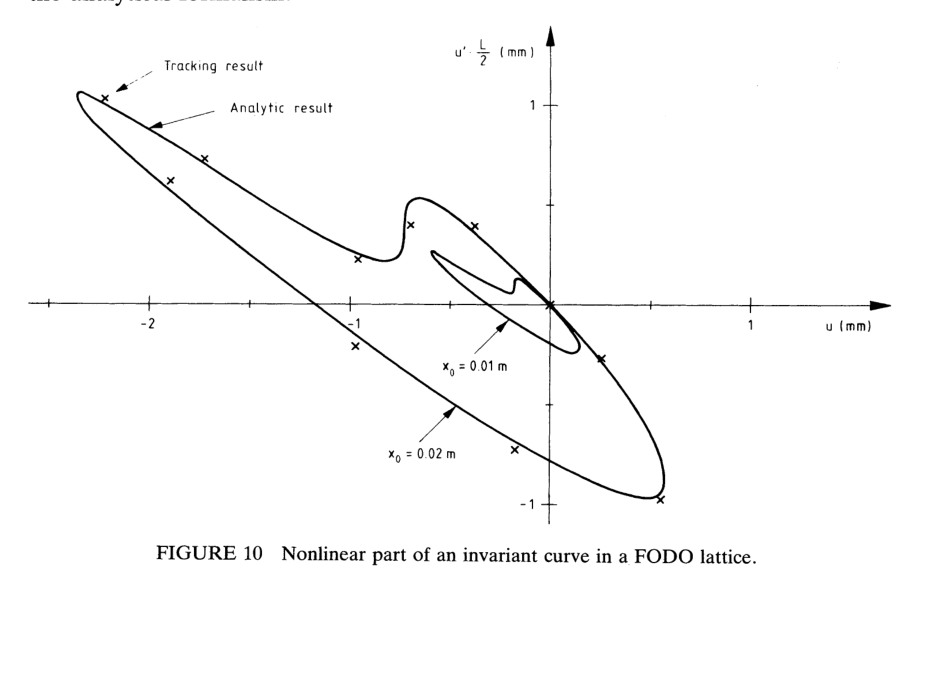
\includegraphics[width=0.78\textwidth]{fig10.png}
\caption{Нелинейная часть инвариантной кривой в FODO-решётке. Сплошная ---
аналитика, кресты --- трекинг; $x_0=0{,}01$~м и $0{,}02$~м.}
\label{fig:10}
\end{figure}

Рис.~\ref{fig:11} показывает полную инвариантную кривую $\mathbf{X}(n)$ вблизи
резонанса третьего порядка. Видна типичная треугольная
форма\textsuperscript{8,9,19}. Аналитические значения снова очень хорошо
согласуются с численными. Результаты --- в нормированных координатах фазового
пространства $(x/\sqrt{\beta},\,x'\sqrt{\beta})$ в центре фокусирующего
квадруполя ($\alpha=-\beta'=0$). Динамическая апертура $x_{\mathrm{lim}}$ равна
$2{,}2$~см.

\begin{figure}[H]
\centering
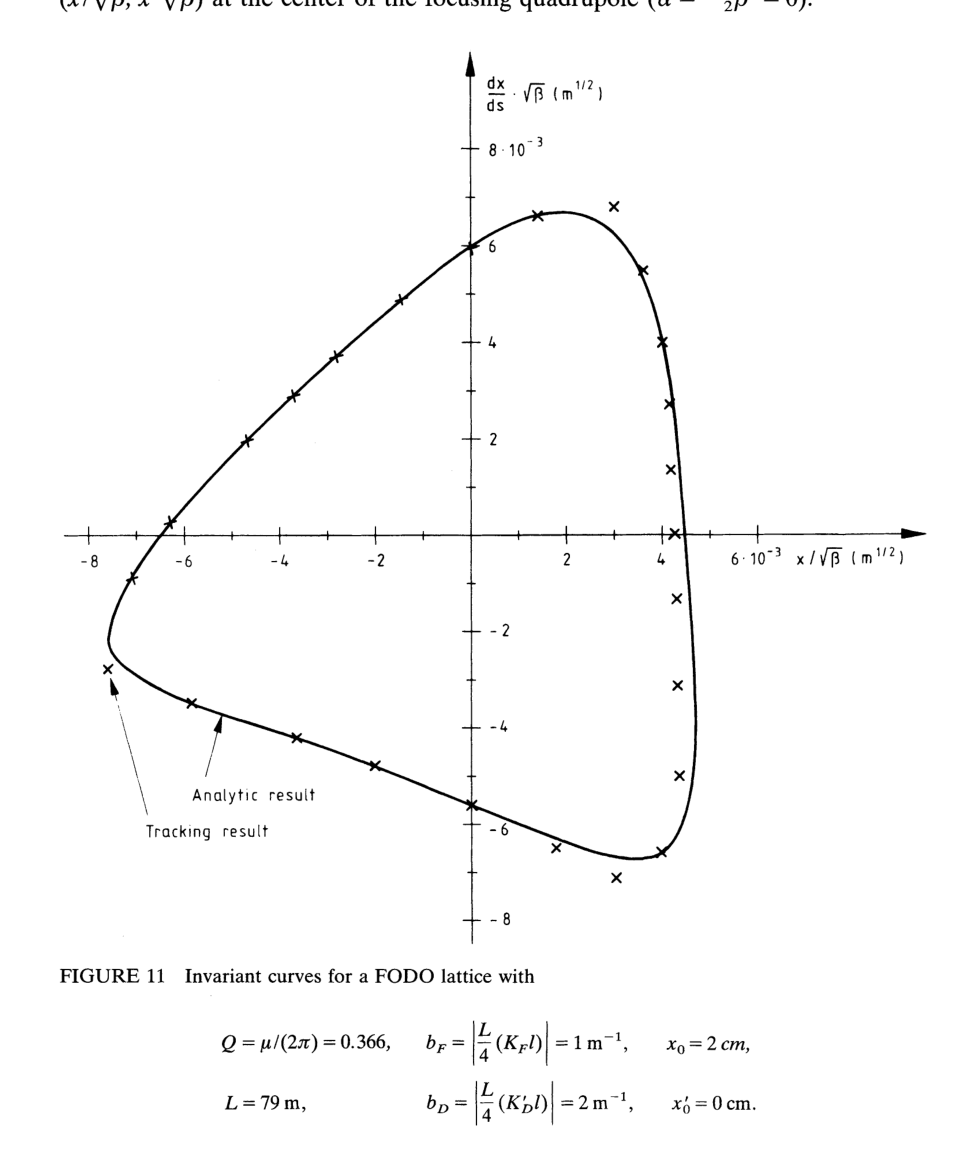
\includegraphics[width=0.82\textwidth]{fig11.png}
\caption{Инвариантные кривые для FODO-решётки с
$Q=\mu/(2\pi)=0{,}366$, $L=79$~м,
$b_F=|(K'_F l)|=1$~м$^{-1}$, $b_D=|(K'_D l)|=2$~м$^{-1}$,
$x_0=2$~см, $x'_0=0$.}
\label{fig:11}
\end{figure}

\subsection{Обобщение на два измерения}

В двух измерениях $(x,z)$ уравнения движения при $\delta=0$ таковы\textsuperscript{17}:
\begin{equation}
x''-k(s)x-\tfrac12 m(s)(x^2-z^2)=0,
\end{equation}
\begin{equation}
z''+k(s)z+m(s)xz=0.
\end{equation}
Предполагается, что линейной связи между двумя движениями нет и связь идёт
только от нелинейных членов секступольных полей. Формализм сразу обобщается:
первая линеаризация обоих уравнений
\begin{equation}
x^{(0)\prime\prime}-k(s)x^{(0)}=0,\qquad
x^{(0)}(0)=x_0,\quad x^{(0)\prime}(0)=x'_0,
\end{equation}
\begin{equation}
z^{(0)\prime\prime}+k(s)z^{(0)}=0,
\end{equation}
с $u^{(0)}(0)=u^{(0)\prime}(0)=0$ и $v^{(0)}(0)=v^{(0)\prime}(0)=0$. Записывая
$x=x^{(0)}+u$, $z=z^{(0)}+v$, после второй линеаризации
\begin{equation}
u^{(0)\prime\prime}-\bigl[k(s)+m(s)x^{(0)}(s)\bigr]u^{(0)}
+m(s)z^{(0)}(s)v^{(0)}
=\tfrac12 m(s)\bigl\{[x^{(0)}]^2-[z^{(0)}]^2\bigr\},
\end{equation}
\begin{equation}
v^{(0)\prime\prime}+\bigl[k(s)+m(s)x^{(0)}(s)\bigr]v^{(0)}
+m(s)z^{(0)}(s)u^{(0)}
=-m(s)x^{(0)}z^{(0)}.
\end{equation}
Снова можно заменить $x^{(0)}$ и $z^{(0)}$ в левых частях их средними. Поскольку
$\langle x^{(0)}\rangle=\langle z^{(0)}\rangle=0$,
\begin{equation}
u^{(0)\prime\prime}-k(s)u^{(0)}=\tfrac12 m(s)\bigl\{[x^{(0)}]^2-[z^{(0)}]^2\bigr\},
\end{equation}
\begin{equation}
v^{(0)\prime\prime}+k(s)v^{(0)}=-m(s)x^{(0)}z^{(0)}.
\end{equation}
Уравнения расцеплены по $u^{(0)}$ и $v^{(0)}$, и каждое можно решать отдельно.
Действуя точно как в §5.1, получаем выражения для $\mathbf{X}(n)$ и
$\mathbf{Z}(n)$. Примеры будут посчитаны и опубликованы позже.

\subsection{Динамическая апертура}

Характерная черта решений нелинейного уравнения бетатронного движения ---
оставаться ограниченными до некоторой амплитуды и затем внезапно становиться
неограниченными. Пороговая амплитуда и называется динамической апертурой
системы. Цель этого раздела --- лучше понять механизмы, движущие этот эффект, и
дать полуаналитический инструмент для поиска приближённых начальных условий,
выше которых движение неограничено (границы устойчивости). Все расчёты --- для
одномерного горизонтального движения, но в принципе обобщаются на два измерения
(это ещё не сделано).

Базовый эффект качественно виден из уравнения движения\textsuperscript{17}:
\begin{equation}
x''-k(s)x-\tfrac12 m(s)x^2=0.
\end{equation}
Начиная с некоторой амплитуды нелинейный член становится доминирующим, и
происходит самоусиление. Это демонстрируется простым примером нелинейного
рекуррентного соотношения
\begin{equation}
x_{n+1}=\lambda x_n^2.
\end{equation}
Его точное решение
\begin{equation}
x_n=x_0(\lambda x_0)^{2^n-1},
\end{equation}
где $x_0$ --- начальное значение. Из~(96) ясно, что $x_n$ остаётся ограниченным,
если
\begin{equation}
|\lambda x_0|<1.
\end{equation}
Иными словами, при $\lambda,x_0>0$ динамическая апертура системы~(95) есть
\begin{equation}
(x_0)_{\mathrm{lim}}=\frac1\lambda.
\end{equation}
Если $x_0$ превосходит это критическое значение, нелинейный член~(95)
доминирует, и происходит быстрое самоусиление. Пока кажется, что эффект
динамической апертуры --- чисто <<эффект большой амплитуды>>, то есть нет надежды
описать его пертурбативными методами. В реальных системах, однако, например в
~(94), границу устойчивости обычно наблюдают при \emph{малых} амплитудах, когда
нелинейный член ещё не доминирует; следовательно, пертурбативные методы должны
быть применимы. Наличие неустойчивости при малых амплитудах указывает на второй
механизм, не описанный простой моделью выше: механизм, который гонит решение к
режиму самоусиления. Чтобы его найти, снова используем метод последовательных
линеаризаций. Уравнение для $u^{(0)}$ после второй линеаризации уже дано ---
это~(64), которое повторим:
\begin{equation}
u^{(0)\prime\prime}-\bigl[k(s)+m(s)x^{(0)}(s)\bigr]u^{(0)}
=\tfrac12 m(s)\bigl[x^{(0)}(s)\bigr]^2,
\tag{64}
\end{equation}
с
\begin{equation}
u^{(0)}(0)=u^{(0)\prime}(0)=0.
\tag{65}
\end{equation}
В приложении~A доказано, что неограниченность~(64) обеспечивается уже
неограниченностью только однородной части:
\begin{equation}
u^{(0)\prime\prime}-\bigl[k(s)+m(s)x^{(0)}(s)\bigr]u^{(0)}=0.
\end{equation}

С другой стороны, из подхода к инвариантным кривым (§5.1) известно, что
неоднородный член даёт неограниченное движение только при отдельных значениях
$\mu$ (резонансы). Поэтому в этом порядке приближения полная информация о
динамической апертуре, вообще говоря, содержится в однородной части [ур.~(99)].
Решение линейного бетатронного движения $x^{(0)}(s)$ входит в коэффициент~(99), и
это вводит зависимость решения $u^{(0)}$ от линейной амплитуды.

Поскольку $u^{(0)}(s)$ вообще не периодично на одном периоде магнитной структуры,
описываемой $m(s)$ и $k(s)$, уравнение~(99) сводится лишь к векторному
рекуррентному соотношению с \emph{непостоянной} транспортной матрицей:
\begin{equation}
\begin{pmatrix}u_{n+1}^{(0)}\\ u_{n+1}^{(0)\prime}\end{pmatrix}
=M_n
\begin{pmatrix}u_n^{(0)}\\ u_n^{(0)\prime}\end{pmatrix}.
\end{equation}
Однако если линейная частота $Q$ структуры рациональна, то есть
\begin{equation}
Q=\frac{p}{q},\qquad p,q\in\mathbb{Z},
\end{equation}
теория работы\textsuperscript{1} и ур.~(63) показывают, что $x^{(0)}(s)$
становится периодическим с периодом, равным $q$ магнитным периодам структуры.
Тогда~(99) --- уравнение Хилла с матрицей, не зависящей от $n$:
\begin{equation}
R=\prod_{i=q-1}^{0} M_i,
\end{equation}
где $M_i$ --- транспортная матрица на $i$-м магнитном периоде, как в~(99).
Линейная теория говорит, что решение $u^{(0)}$ ограничено, если
\begin{equation}
\bigl|\Tr R\bigr|<2.
\end{equation}

Заметим, что $R$ явно содержит начальные условия $x_0$ и $x'_0$, как видно из
~(99). Следовательно, условие ограниченности становится функцией $x_0$ и $x'_0$
и может непосредственно использоваться для оценки границы устойчивости.

Теперь ясно, что второй механизм, движущий нелинейные неустойчивости, ---
параметрический резонанс, вызванный <<флуктуирующими транспортными матрицами>> в
возмущающем уравнении для $u^{(0)}$ [ур.~(99)]. Этот резонанс может возникать при
малых амплитудах, гоня решение к большим амплитудам, где затем берёт верх эффект
самоусиления.

Краткий алгоритм поиска приближённой границы устойчивости при заданных $Q$,
$x_0$ и $x'_0$:

\begin{enumerate}
\item[(i)] Приблизить $Q$ рациональным $p/q$ с возможно меньшим $q$.
\item[(ii)] Вычислить матрицу
\begin{equation}
R=\prod_{i=q-1}^{0} M_i.
\end{equation}
\item[(iii)] Посчитать $|\Tr R|$ и потребовать $|\Tr R|<2$.
\end{enumerate}

Для сложной структуры и большого $q$ получать замкнутые выражения для
произведения матриц в~(104) всё труднее и утомительнее. Тем не менее этот метод,
сводящийся к произведению конечного числа матриц при $q\lesssim 100$, даёт
большое преимущество перед трекингом многих частиц на очень большое число
периодов. Это особенно ясно для протонных пучков (нет затухания) и во всех
случаях означает экономию машинного времени.

В качестве примера берём FODO-решётку типа LEP с двумя семействами секступолей
SF и SD у квадруполей F и D. Варьируем $Q=\mu_{\mathrm{cell}}/(2\pi)$ от
$0{,}25$ ($=30/120$) до $0{,}417$ ($=50/120$). Согласно~(102) матрицы $M_i$ тогда
\begin{equation}
M_i=
\begin{pmatrix}
1 & 1 \\
-a-2b_F x_{i+1}^{(0)F} & 1-a-2b_F x_{i+1}^{(0)F}
\end{pmatrix}
\begin{pmatrix}
1 & 1 \\
a+2b_D x_i^{(0)D} & 1+a+2b_D x_i^{(0)D}
\end{pmatrix},
\end{equation}
где
\begin{equation}
b_{F,D}=\frac{L}{4}(K'_{F,D}\,l_{F,D})
\end{equation}
и
\begin{equation}
a=2\sin(\pi Q),
\end{equation}
а $L$ --- длина магнитного периода, $x_i^{(0)D}$ и $x_i^{(0)F}$ --- линейные
бетатронные значения на квадруполях F и D после $i$-го оборота. Матрицы $M_i$
получены из однородного~(99) и имеют в точности вид транспортной матрицы
FODO-решётки, если заменить $k(s)$ на $k(s)+m(s)x^{(0)}(s)$. Кроме того,
независимую координату $s$ заменяют на $s^*=(2/L)s$\textsuperscript{23}. Условие
\begin{equation}
\Biggl|\Tr\prod_{i=119}^{0} M_i\Biggr|<2
\end{equation}
даёт кривую $(x_0)_{\mathrm{lim}}=F(Q)$ --- максимальное начальное значение, при
котором $u^{(0)}$ ещё ограничено. Рис.~\ref{fig:12} показывает $\Tr R(x_0)$ для
$Q=42/120=7/20$. Кривая пересекает линию $\Tr R=-2$ при $x_0=0{,}015$~м, тогда
как ожидаемый предел (численный счёт) есть $x_0=0{,}013$~м. На рис.~\ref{fig:13}
полная кривая $(x_0)_{\mathrm{lim}}=F(Q)$ сравнивается с ожидаемым пределом и с
пределом по неподвижным точкам резонанса\textsuperscript{8,9,19}, вычислимым
вблизи резонанса третьего порядка ($Q=\tfrac13$). Ожидаемый предел найден счётом
точного нелинейного преобразования этой задачи\textsuperscript{24} на $10^5$
периодов с увеличением $x_0$ шагами по 1~мм, пока не достигнута неограниченность
(переполнение). Устойчивость означает тогда $x(10^5)-x(10^4)<1$~мм.

Отчётливо видны резонансы четвёртого и третьего порядка (нулевая граница
устойчивости). Согласие ожидаемого предела с пределом по условию следа~(108)
очень хорошее в диапазоне $Q$ от $36/120$ до $50/120$. Для
$Q=30/120$--$35/120$ согласие хуже. Подозреваем, что это из-за линеаризации
уравнения для $u$, эквивалентной пренебрежению перекрёстными членами между силами
SF и SD, важными для резонансов более высокого порядка. Как и ожидалось,
трактовка неподвижных точек третьего порядка (насколько нам известно ---
единственная аналитическая трактовка динамической апертуры до сих пор) быстро
ломается, если фактическое $Q$ слишком далеко от $Q=1/3$.

\begin{figure}[H]
\centering
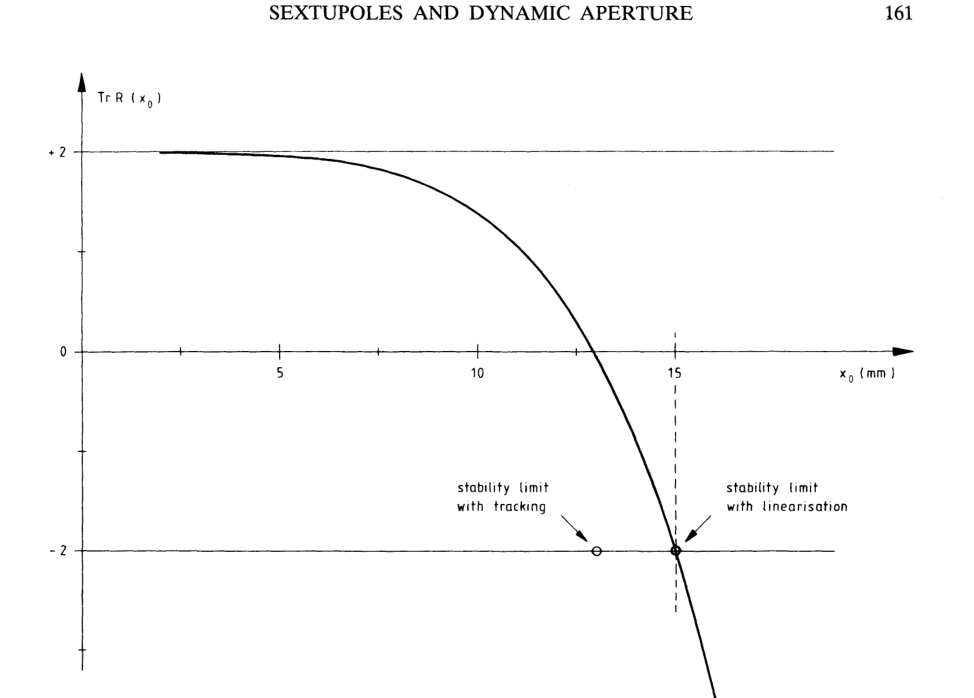
\includegraphics[width=0.88\textwidth]{fig12.png}
\caption{Граница устойчивости для FODO-решётки с $Q=7/20=0{,}35$:
$L_{\mathrm{cell}}=79$~м, $K'_F=-0{,}127$~м$^{-3}$, $K'_D=0{,}133$~м$^{-3}$.}
\label{fig:12}
\end{figure}

\begin{figure}[H]
\centering
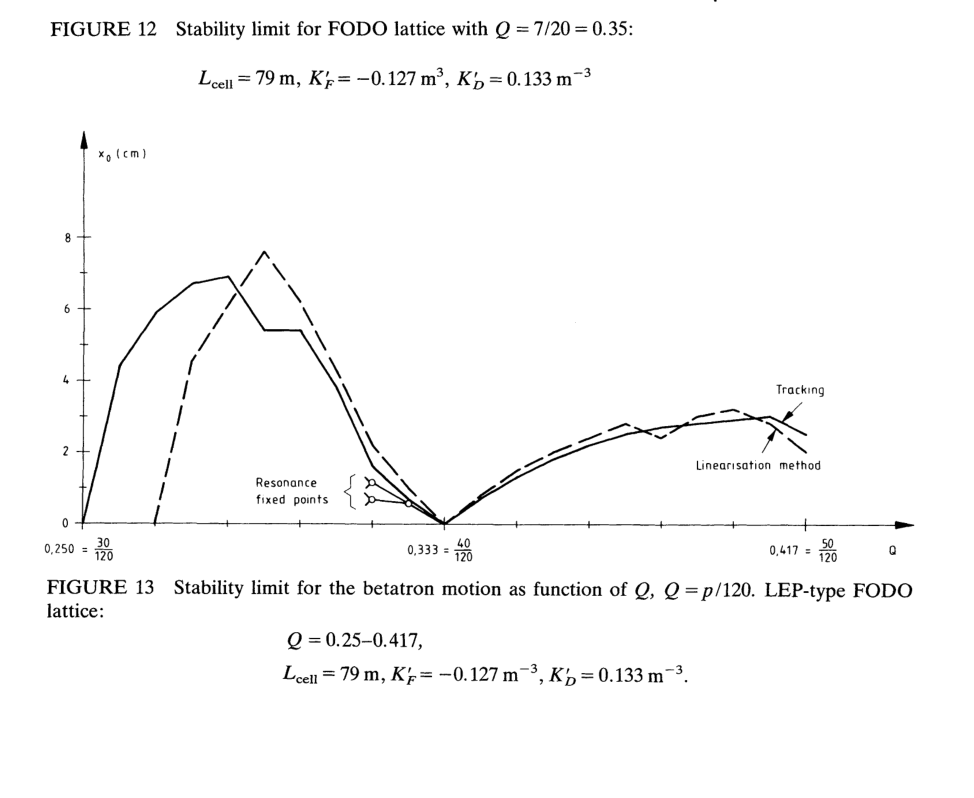
\includegraphics[width=0.92\textwidth]{fig13.png}
\caption{Граница устойчивости бетатронного движения как функция $Q$,
$Q=p/120$. FODO-решётка типа LEP: $Q=0{,}25$--$0{,}417$,
$L_{\mathrm{cell}}=79$~м, $K'_F=-0{,}127$~м$^{-3}$, $K'_D=0{,}133$~м$^{-3}$.}
\label{fig:13}
\end{figure}

\begin{thebibliography}{26}
\bibitem{1}
E.~D. Courant and H.~S. Snyder, \textit{Ann.\ Phys.\ (NY)} \textbf{3}, 1 (1958).
\bibitem{2}
R.~A. Beck, R.~Belbeoch, and G.~Gendreau, in \textit{Proceedings of the Conference
on High Energy Accelerators}, Cambridge (1967) p.~A-63.
\bibitem{3}
B.~W. Montague, \textit{Linear Optics for Improved Chromaticity Correction},
LEP Note 165 (1979).
\bibitem{4}
B.~Autin and A.~Verdier, \textit{Focussing Perturbations in Alternating Gradient
Structures}, CERN ISR-LTD/76-14 (1976).
\bibitem{5}
G.~Guignard, \textit{First Order Chromatic Perturbations and Sextupole Strength},
CERN ISR-TH/82-14 (1982).
\bibitem{6}
\textit{LEP Design Report, Vol.~II, The LEP Main Ring}, CERN/LEP/84-01 (1984).
\bibitem{7}
G.~Guignard and A.~Verdier, \textit{Description of the LEP Lattice Version 13,
Configuration with $60^\circ$ in the Arc Cells}, CERN LEP-TH/83-53 (1983).
\bibitem{8}
G.~Guignard, \textit{Effets des champs magnétiques perturbateurs d'un synchrotron
sur l'orbite fermée et les oscillations bétatroniques, ainsi que leur
compensation}, CERN 70-24 (1970).
\bibitem{9}
R.~Hagedorn, \textit{Stability and Amplitude Ranges of Two Dimensional Non-linear
Oscillations with Periodical Hamiltonian}, CERN 57-1 (1957).
\bibitem{10}
K.~L. Brown and R.~V. Servranckx, \textit{IEEE Trans.\ Nucl.\ Sci.}
\textbf{NS-26}, 3598 (1979).
\bibitem{11}
A.~Verdier, in \textit{Proceedings of the 12th International Conference on High
Energy Accelerators}, Fermilab (1983).
\bibitem{12}
A.~Verdier, \textit{Influence of the Vertical Phase of the Sextupoles and Their
Number on the Chromaticity Correction of LEP 13}, LEP Note 473 (1983).
\bibitem{13}
A.~Verdier, \textit{Optimisation of the Sextupole Scheme for the Chromaticity
Correction of LEP 13 with $90^\circ$ per Cell}, LEP Note 503 (1984).
\bibitem{14}
M.~Donald, \textit{Chromaticity Correction in Circular Accelerators and Storage
Rings, Part 1: A User's Guide to the HARMON Programs}, PEP Note 311 (1979).
\bibitem{15}
G.~Guignard, \textit{Analytical Calculation of the Sextupole Strengths in LEP
Version 13}, LEP Note 457 (1983).
\bibitem{16}
F.~C. Iselin, in \textit{Proceedings of the 12th International Conference on High
Energy Accelerators}, Fermilab (1983).
\bibitem{17}
H.~Wiedemann, \textit{Chromaticity Correction in Large Storage Rings}, PEP Note
220 (1976); H.~Wiedemann, \textit{User's Guide for PATRICIA}, PEP Technical Memo
PTM-230 (1981).
\bibitem{18}
E.~D. Courant et al., in \textit{Physics of High Energy Particle Accelerators},
AIP Conf.\ Proc.\ 87 (1981).
\bibitem{19}
A.~Schoch, \textit{Theory of Linear and Non-linear Perturbations of Betatron
Oscillations in Alternating Gradient Synchrotrons}, CERN 57-23 (1958).
\bibitem{20}
G.~Guignard, \textit{A General Treatment of Resonances in Accelerators}, CERN
78-11 (1978).
\bibitem{21}
A.~Ando, \textit{Particle Accelerators} \textbf{15}, 177 (1984).
\bibitem{22}
T.~L. Collins, \textit{Distortion Functions}, Fermilab-84/114 (1984).
\bibitem{23}
J.~Hagel, \textit{Analytic Calculation of the Off-Momentum Closed Orbit in Storage
Rings with Insertions and Sextupoles}, CERN/LEP-TH/84-18 (1984).
\bibitem{24}
J.~Hagel, \textit{Single Particle Theory of AG-Synchrotrons Taking into Account
Momentum Dependence and Non-linearities of the Focussing Force}, диссертация,
Technical University of Graz (1984).
\bibitem{25}
L.~Berg, \textit{Differenzengleichungen zweiter Ordnung mit Anwendungen}, UTB 906
(1979).
\bibitem{26}
Bronstein--Semendjajew, \textit{Taschenbuch der Mathematik} (Verlag Harri Deutsch,
1981).
\end{thebibliography}

\appendix
\section{Неограниченность неоднородного уравнения}

Докажем следующее следствие. Если все однородные решения уравнения
\begin{equation}
u''+a(s)u=b(s)
\end{equation}
неограничены, то по крайней мере решение неоднородного уравнения с начальными
условиями $u(0)=u'(0)=0$ будет неограниченным.

\textit{Доказательство.} Решение~(A-1) с указанными начальными условиями можно
записать в интегральной форме\textsuperscript{26}
\begin{equation}
u(s)=u_{HC}(s)\int_0^s u_{HS}(\sigma)b(\sigma)\,d\sigma
-u_{HS}(s)\int_0^s u_{HC}(\sigma)b(\sigma)\,d\sigma,
\end{equation}
где $u_{HC}(s)$ и $u_{HS}(s)$ --- решения \emph{однородного} уравнения,
отвечающего~(A-1), с начальными условиями
\begin{equation}
\begin{aligned}
u_{HC}(0)&=1,& u'_{HC}(0)&=0,\\
u_{HS}(0)&=0,& u'_{HS}(0)&=1.
\end{aligned}
\end{equation}
Функции $u_{HC}$ и $u_{HS}$ часто называют косинусоподобной и синусоподобной.
Уравнение~(A-2) в векторной записи:
\begin{equation}
u(s)
=\begin{pmatrix}u_{HC}\\ -u_{HS}\end{pmatrix}
\cdot
\int_0^s b(\sigma)
\begin{pmatrix}u_{HS}\\ u_{HC}\end{pmatrix}\,d\sigma
=\mathbf{V}_1\cdot\mathbf{V}_2.
\end{equation}
Если предположить, что $u(s)$ ограничено, а $u_{HS}$ и $u_{HC}$ --- нет, векторы
$\mathbf{V}_1$ и $\mathbf{V}_2$ в~(A-4) должны быть ортогональны, чтобы их
скалярное произведение оставалось конечным.

Поскольку начальные векторы
\[
\begin{pmatrix}u_{HC}\\ -u_{HS}\end{pmatrix}
\quad\text{и}\quad
\begin{pmatrix}u_{HS}\\ u_{HC}\end{pmatrix}
\]
перпендикулярны, это означает, что интегрирование в~(A-4) не должно менять
направления содержащегося в нём вектора. Следовательно,
\begin{equation}
\int_0^s b(\sigma)
\begin{pmatrix}u_{HS}\\ u_{HC}\end{pmatrix}\,d\sigma
=\lambda
\begin{pmatrix}u_{HS}\\ u_{HC}\end{pmatrix},
\end{equation}
где $\lambda$ --- произвольная вещественная константа.

Дифференцируя~(A-5) один раз по $s$, получаем два дифференциальных уравнения
первого порядка для $u_{HS}$ и $u_{HC}$. Но из вида~(A-5) ясно, что $u_{HS}$ и
$u_{HC}$ не зависят от коэффициентной функции $a(s)$. Это противоречит однородной
части~(A-1), решениями которой по определению и являются $u_{HS}$ и $u_{HC}$.
Поэтому~(A-5) не может выполняться для $u_{HS}$ и $u_{HC}$ в общем случае, и
$u(s)$ необходимо станет неограниченным, если неограничены $u_{HS}$ и $u_{HC}$.
Следствие доказано.

\section{Векторы A, B, C для тонкого секступоля}

Выведем $\mathbf{A}$, $\mathbf{B}$ и $\mathbf{C}$ из рекуррентного соотношения
[ур.~(69)] на примере структуры из дрейфов и квадруполей в произвольном порядке
и одного тонкого секступоля силы $K'$ в положении $s=j$. Базовое уравнение
[ур.~(67)] есть
\begin{equation}
u''-k(s)u=\tfrac12 m(s)\bigl[x^{(0)}(s)\bigr]^2.
\end{equation}
Всюду, кроме точки $s=j$, это в точности уравнение линейного бетатронного
движения, и преобразование вектора $(u,u')$ между двумя точками, не содержащими
$s=j$, даётся линейными транспортными матрицами. Преобразование от входа к выходу
тонкого секступоля получается интегрированием~(B-1) по интервалу
$(j-\varepsilon,j+\varepsilon)$ при $\varepsilon\to 0$:
\begin{equation}
u'_{\mathrm{exit}}-u'_{\mathrm{ent}}
=\tfrac12\int_{j-\varepsilon}^{j+\varepsilon}m(s)\bigl[x^{(0)}(s)\bigr]^2\,ds
=\tfrac12(K'l)\bigl[x_j^{(0)}\bigr]^2.
\end{equation}
Здесь $(K'l)$ --- интегральная сила секступоля. Кроме того, должна выполняться
непрерывность
\begin{equation}
u_{\mathrm{exit}}=u_{\mathrm{ent}},
\end{equation}
так что полное преобразование
\begin{equation}
\begin{pmatrix}u\\ u'\end{pmatrix}_{\mathrm{exit}}
=
\begin{pmatrix}u\\ u'\end{pmatrix}_{\mathrm{ent}}
+\tfrac12(K'l)\bigl[x_j^{(0)}\bigr]^2
\begin{pmatrix}0\\ 1\end{pmatrix}.
\end{equation}

Рассмотрим преобразование вектора за полную структуру от оборота $n$ к обороту
$n+1$. Определим матрицы $M_{0,j}$ и $M_{j,1}$ как постоянные (не зависящие от
$n$) матрицы от начала структуры до секступоля $s=j$ и от $s=j$ до конца
структуры. Разумеется,
\begin{equation}
M_{0,1}=M_{0,j}\,M_{j,1}=M,
\end{equation}
где $M$ --- транспортная матрица полной структуры. Нужно применить последовательные
преобразования:

\begin{enumerate}
\item[(i)] От начала структуры до входа секступоля:
\begin{equation}
\mathbf{U}_{j-\varepsilon}=M_{0,j}\mathbf{U}_n.
\end{equation}
\item[(ii)] Через секступоль:
\begin{equation}
\mathbf{U}_{j+\varepsilon}
=\mathbf{U}_{j-\varepsilon}
+\tfrac12(K'l)\bigl[x_j^{(0)}\bigr]^2
\begin{pmatrix}0\\ 1\end{pmatrix}.
\end{equation}
\item[(iii)] От выхода секступоля до конца структуры:
\begin{equation}
\mathbf{U}_{n+1}=M_{j,1}\mathbf{U}_{j+\varepsilon}.
\end{equation}
\end{enumerate}

Из (i)--(iii) полное преобразование:
\begin{equation}
\mathbf{U}_{n+1}
=M\mathbf{U}_n
+\tfrac12(K'l)\bigl[x_j^{(0)}\bigr]^2
M_{j,1}\begin{pmatrix}0\\ 1\end{pmatrix}.
\end{equation}
Величину $x_j^{(0)}$ в~(B-10) можно выразить как
\begin{equation}
x_j^{(0)}=\bigl\{M_{0,j}\mathbf{X}_n^{(0)}\bigr\}_1,
\end{equation}
где $\{\,\}_1$ означает первую компоненту вектора в скобках. Пользуясь~(63) для
$\mathbf{X}_n^{(0)}$, находим
\begin{equation}
\bigl[x_j^{(0)}\bigr]^2=\alpha\cos(2n\mu)+\beta\sin(2n\mu)+\gamma,
\end{equation}
где
\begin{equation}
\alpha=\tfrac12\Biggl(
\bigl\{M_{0,j}\mathbf{X}_0\bigr\}_1^2
-\frac{\bigl\{M_{0,j}(M-I\cos\mu)\mathbf{X}_0\bigr\}_1^2}{\sin^2\mu}\Biggr),
\end{equation}
\begin{equation}
\beta=\bigl\{M_{0,j}\mathbf{X}_0\bigr\}_1
\frac{\bigl\{M_{0,j}(M-I\cos\mu)\mathbf{X}_0\bigr\}_1}{\sin\mu},
\end{equation}
\begin{equation}
\gamma=\tfrac12\Biggl(
\bigl\{M_{0,j}\mathbf{X}_0\bigr\}_1^2
+\frac{\bigl\{M_{0,j}(M-I\cos\mu)\mathbf{X}_0\bigr\}_1^2}{\sin^2\mu}\Biggr).
\end{equation}
Подставляя~(B-13)--(B-15) в~(B-10), окончательно получаем
\begin{equation}
\mathbf{U}_{n+1}=M\mathbf{U}_n
+\mathbf{A}\cos(2n\mu)+\mathbf{B}\sin(2n\mu)+\mathbf{C},
\end{equation}
где
\begin{equation}
\mathbf{A}=\tfrac12\alpha(K'l)\,M_{j,1}\begin{pmatrix}0\\ 1\end{pmatrix},
\end{equation}
\begin{equation}
\mathbf{B}=\tfrac12\beta(K'l)\,M_{j,1}\begin{pmatrix}0\\ 1\end{pmatrix},
\end{equation}
\begin{equation}
\mathbf{C}=\tfrac12\gamma(K'l)\,M_{j,1}\begin{pmatrix}0\\ 1\end{pmatrix}.
\end{equation}

\end{document}

